\documentclass[12pt]{article}
\usepackage[utf8]{inputenc}
\usepackage{lmodern}
\usepackage[T1]{fontenc}
\usepackage{amsmath}
\usepackage{enumitem}
\usepackage{graphicx}
\usepackage{fullpage}
\usepackage{siunitx}
\usepackage{fancyhdr}
\PassOptionsToPackage{hyphens}{url}
\usepackage[hyphens]{url}
\usepackage{color}
% \usepackage[options]{algorithm2e}
\usepackage{enumitem}
\usepackage{textcomp}
\usepackage{geometry}
\usepackage{courier}
\usepackage{listings}
\usepackage{array}
\usepackage{amsthm}
\usepackage{mathdots}
\usepackage{amssymb}
% \usepackage{minted}
\usepackage{wrapfig}
\usepackage{titlesec}
\usepackage{parskip}
\usepackage{accents}
\usepackage{gensymb}
\usepackage{indentfirst}
\usepackage{courier}
\usepackage{framed}
\usepackage{etoolbox}
\usepackage{titlesec}
\usepackage{appendix}
\usepackage{mdframed}
\usepackage{verbatim}
\usepackage{xspace}
\usepackage{hyperref}
\usepackage{todonotes}
\AtBeginEnvironment{subappendices}{%
\section*{Appendix}
\addcontentsline{toc}{section}{Appendices}
}



\newcommand{\mytitle}{\textbf{inzva Algorithm Programme 2018-2019\\ \ \\Bundle 10 \\ \ \\ Math-3 (Geometry)}}
\title{\vspace{-2em}\mytitle\vspace{-0.3em}}
\author{\textbf{Editor}\\Yusuf Hakan Kalaycı\\ \ \\ \textbf{Reviewer} \\Hasan Bal}





%\lstset{language=C++,
%                basicstyle=\ttfamily,
%                keywordstyle=\color{blue}\ttfamily,
%                stringstyle=\color{red}\ttfamily,
%                commentstyle=\color{green}\ttfamily,
%                morecomment=[l][\color{magenta}]{\#}
%}

\definecolor{keywordcolor}{rgb}{0,0,0.45}
\definecolor{stringcolor}{rgb}{0.45,0.45,0.45}
\definecolor{commentcolor}{rgb}{0,0.3,0}

\lstset{
language=C++,
basicstyle=\footnotesize\ttfamily,
numbers=left,
%numberstyle=\tiny,
frame=tb,
columns=fullflexible,
showstringspaces=false,
breaklines=true,
tabsize=4,
keywordstyle=\color{keywordcolor}\footnotesize\bf\ttfamily,
stringstyle=\color{stringcolor}\footnotesize\ttfamily,
commentstyle=\color{commentcolor}\it\sffamily
}
% \lstset{basicstyle=\ttfamily,breaklines=true}
\lstloadlanguages{C++}

%\renewcommand{\familydefault}{\sfdefault}

\addtolength{\parskip}{\baselineskip}  
\newcommand{\urlwofont}[1]{\urlstyle{same}\url{#1}}

\renewcommand{\arraystretch}{0.8}
\renewcommand{\headrulewidth}{0pt}
\renewcommand{\footrulewidth}{0pt}

\newcommand{\imagewidth}{0.8\textwidth}

\lhead{}
\chead{}
\rhead{}
\lfoot{}
\cfoot{\thepage}
\rfoot{}

\geometry{
  top=0.9in,
  inner=0.7in,
  outer=0.7in,
  bottom=0.9in,
  headheight=2ex,
  headsep=1ex,
}
\pagestyle{fancy}
%\fancyhf{}
%\setlength{\headsep}{0.2in}


\fancypagestyle{firststyle}
{
    \chead{}
    \setlength{\headsep}{0.0in}
}
\hypersetup{
    unicode=true,
    colorlinks=true,
    linkcolor=blue,
    citecolor=black,
    filecolor=black,
    urlcolor=blue
}

\begingroup
    \makeatletter
    \@for\theoremstyle:=definition,remark,plain\do{%
        \expandafter\g@addto@macro\csname th@\theoremstyle\endcsname{%
            \addtolength\thm@preskip\parskip
            }%
        }
\endgroup

\newtheorem{thm}{Theorem}[section]
\newtheorem{lemma}{Lemma}[section]
\newtheorem{claim}{Claim}[section]
\newtheorem{defn}{Definition}[section]
\newtheorem{proposition}{Proposition}[section]
\newtheorem{exercise}{Exercise}[section]
\newtheorem{example}{Example}[section]
\newtheorem{corollary}{Corollary}[section]
\newtheorem{remark}{Remark}[section]
%\theoremstyle{empty}
\newtheorem*{namedthm}{Theorem}


% indention size
%\setlength{\parindent}{19pt}
\setlength{\parindent}{0pt}

% paragraph spacing
\setlength{\parskip}{1em}

% line spacing
\linespread{1}

%\setcounter{tocdepth}{1}

\date{}
\begin{document}

\begin{figure}
  \centering
  
\includegraphics[width=\linewidth/4]{inzva-logo.png}
  \label{fig:inzva}
\end{figure}
\maketitle

\cleardoublepage
\tableofcontents
\markboth{Table of Contents}{}
\cleardoublepage
% \newcommand{\sectionbreak}{\clearpage}

% math tools
\newcommand{\R}{\mathbb{R}}

\section{Introduction}
In this lecture, we will work on a set of well-studied problems gaining their nature from geometry. We will start with the fundamentals of computational geometry, such as vectors, distances, and vector products. Based on these fundamentals we will define
our first primitives such as area calculation methods, distance methods, and intersection methods. With the help of these primitives we will study the following:
\begin{itemize}
    \item Inclusion Problem: whether a point is inside a polygon or not.
    \item Convex Hull: finding the minimum convex polygon containing all given points.
    \item Rotating Calipers Method: a tool to find the farthest pair of points.
    \item Closest Pair: finding the closest pair of given $n$ points.
    \item Applications of Line-Sweep Method: a very useful technique for approaching
    many geometry problems.
\end{itemize}

The reason why we keep Vector Calculus section sufficiently long is that understanding the
nature of the space helps to understand many problems. It is strongly recommended to
think about exercises.

Lastly, Section 2 is prepared using [1] and it closely follows that reference. Section 3,4,5,6 and 7 are prepared using [4] and implementations of the algorithms given in these sections are taken from this website. Also, this reference consists of efficient implementations of many methods and their detailed discussions. Section 8 is prepared using [8]; one might check this reference to see detailed discussions of many applications. The two methods mentioned in Section 9 are designed using [9] and [11] respectively.

\section{Vector Calculus and Analytic Geometry}

\subsection{The Euclidean 3-space or $\R^3$}
\begin{defn}[The Euclidean 3-space]
  The Euclidean 3-space denoted by $\R^3$ is the set 
  $$ \{ (x,y,z) | x,y,z \in \R \} $$
\end{defn}

To specify the location of a point in $\R^3$ geometrically, we use the right-handed
rectangular coordinate system in which three mutually perpendicular coordinate axes meet at the origin.
It is common to use the $x$ and $y$ axes to represent the horizontal coordinate plane and the
$z$-axis for the vertical height.

\begin{center}
\begin{figure}[h]
  \centering
  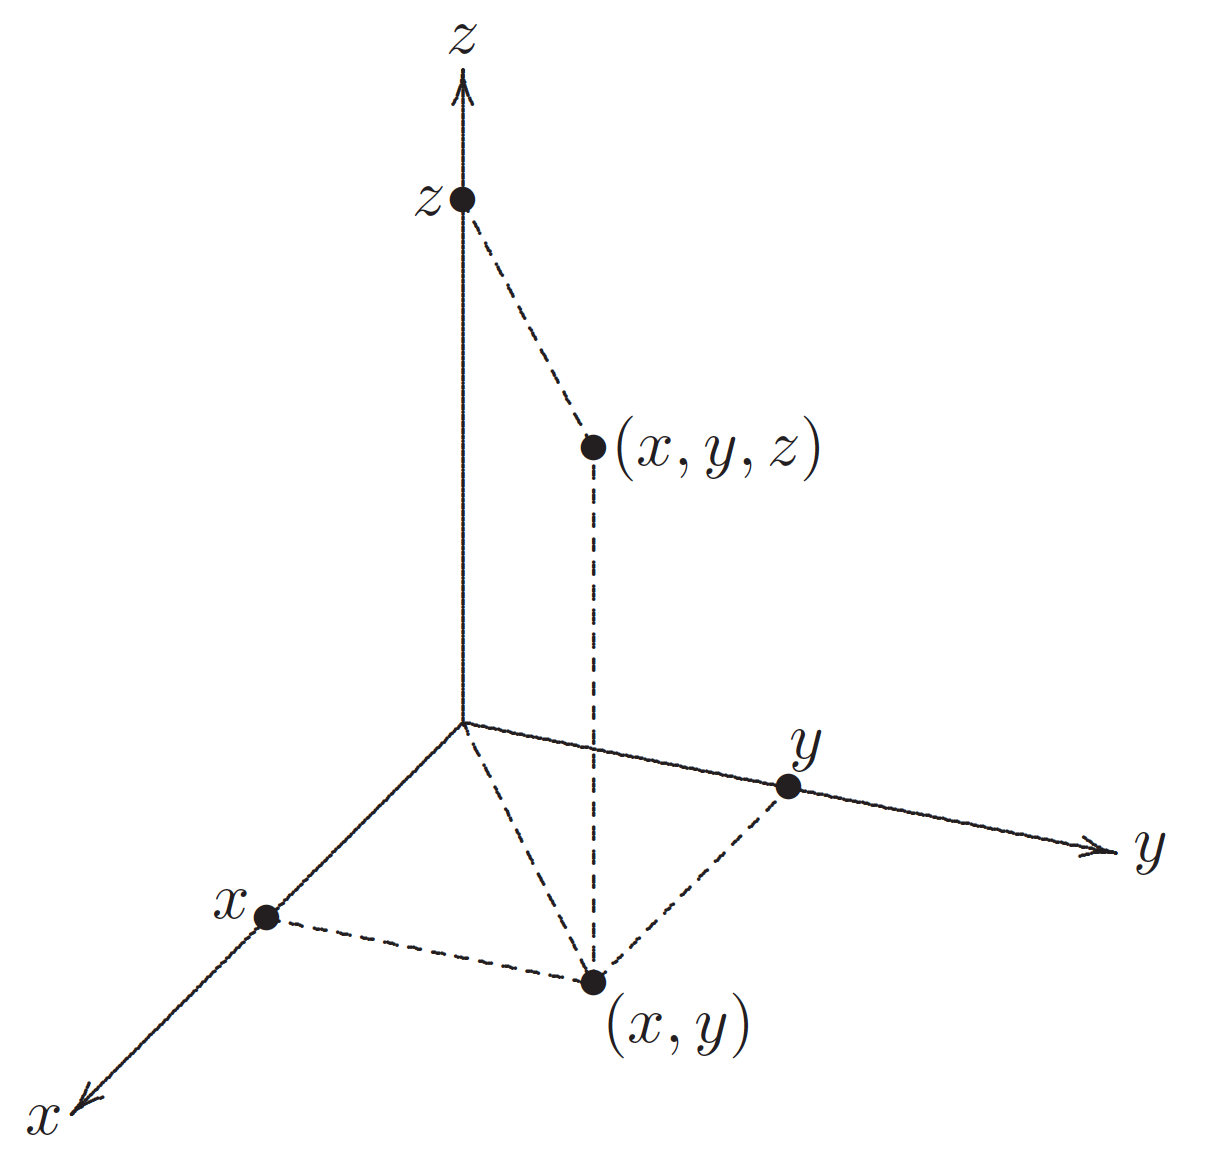
\includegraphics[width=\linewidth/3]{figures/fig1.png}
  \label{fig:1}
  \caption{Representation of points in $R^3$}
\end{figure}
\end{center}

We usually denote a point $P$ with coordinates $(x,y,z)$ by $P(x,y,z)$. The distance
$d(P_1, P_2)$ between two points $P_1(x_1,y_1,z_1)$ and $P_2(x_2,y_2,z_2)$ is given by
$$ d(P_1, P_2) = \sqrt{ (x_1 - x_2)^2 + (y_1 - y_2)^2 + (z_1 - z_2)^2 } $$

The following definition and exercise are out of our scope but they can still be inspiring. The definition involves an abstract notion of our euclidean geometry by [3].

\begin{defn}[Metric Space]
  A metric space is ordered pair $(X,d)$ where $X$ is a set and d is a 
  metric(distance measure) on X such that for any $x,y,z \in X$, the following holds
  \begin{enumerate}
    \item $d(x,y) \geq 0$ \quad \quad \quad \quad \quad \quad \quad (non-negativity)
    \item $d(x,y) = 0 \iff x=y$ \quad 
    \item $d(x,y) = d(y,x)$ \quad \quad \quad \quad \quad (symmetry)
    \item $d(x,z) \leq d(x,y) + d(y,z)$ \quad (sub-additivity or triangle inequality)
  \end{enumerate}
\end{defn}

We are challenging a curious reader with the following exercise.

\begin{exercise}
  Show that $\R^3$ is a metric space with euclidean metric.
\end{exercise}

An equation in $x,y$ and, $z$ describes a surface in $\R^3$. Let us look at some 
standard examples of surfaces.

\begin{example}
(a) $z = 3$ is the equation of a horizontal plane at level 3 above the xy-plane.
(b) $y = 2 $ is the equation of a vertical plane parallel to the xz-coordinate plane. Every point of
this plane has y coordinate equal to 2. (c) Similarly $x = 2$ is the eqaution of a vertical plane
parallel to the yz-coordinate plane.
\end{example}

\begin{center}
  \begin{figure}[h]
    \centering
    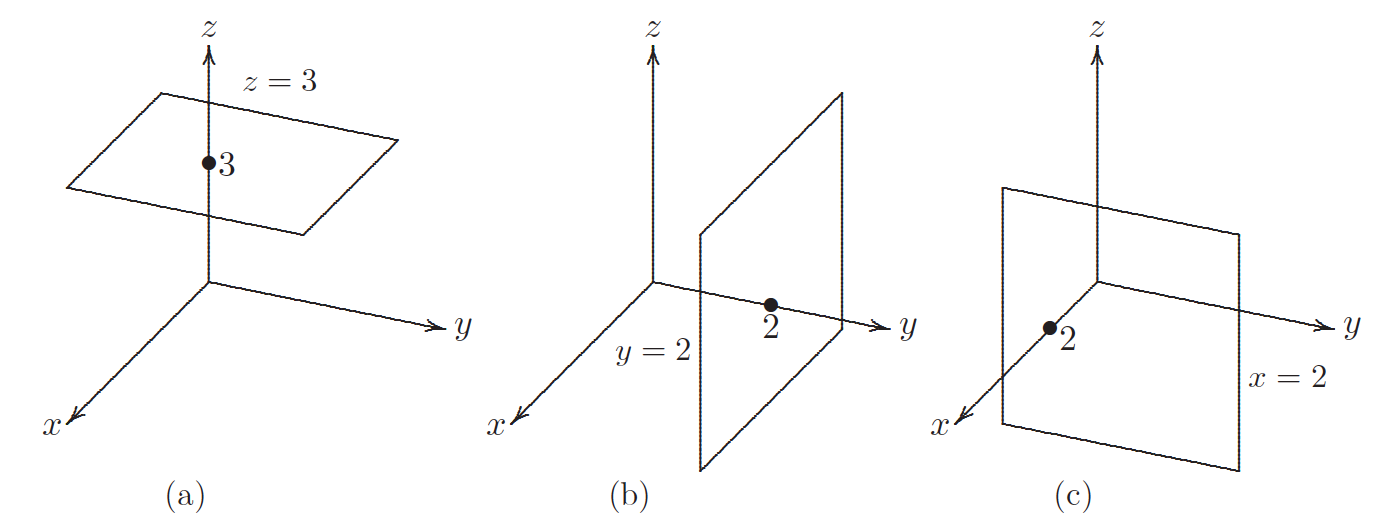
\includegraphics[width=.8\linewidth]{figures/fig2.png}
    \label{fig:2}
    \caption{Planes perpendicular to standard basis}
  \end{figure}
\end{center}

\begin{example}
  An equation of a sphere with centre $O(a, b, c)$ and radius $r$ is !!!!!!!!
\end{example}

\begin{center}
  \begin{figure}[h]
    \centering
    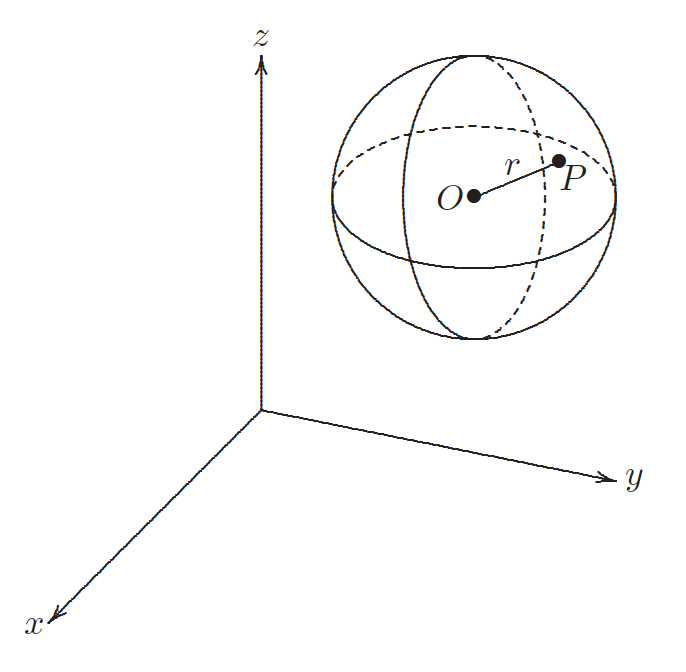
\includegraphics[width=\linewidth/3]{figures/fig3.png}
    \label{fig:3}
    \caption{An example of surface in $R^3$}
  \end{figure}
\end{center}

\subsection{Vectors}

A $3$-dimensional vector is an ordered triple $\pmb{a} = (a_1, a_2, a_3)$ of reals.
We will call $a_1, a_2, a_3$ as components of $\pmb{a}$. Sometimes we can use $\pmb{PQ}$
to denote a vector from a point $P$ to a point $Q$. In $\R^3$, there are some special
vectors which will have special names and can be listed as
\begin{itemize}
  \item $\pmb{i} = (1,0,0)$
  \item $\pmb{j} = (0,1,0)$
  \item $\pmb{k} = (0,0,1)$
\end{itemize}

These vectors $\pmb{i}, \pmb{j}$ and $\pmb{k}$ consist of our standard basis vectors. 
Before we show the importance of those vectors, let's define our addition and multiplication
operators which enable us to work on a vector space(what is it?). Vector addition of two 
vectors $\pmb{u}$ and $\pmb{v}$ is defined as the entrywise addition of their components. Or more formally,
$$\pmb{u}+\pmb{v} = (u_1+v_1, u_2+v_2, u_3+v_3).$$
Multiplication of a vector and a scalar is defined as 
$$ \lambda \pmb{v} = (\lambda v_1, \lambda v_2, \lambda v_3) $$
Then using definitions given above we can decompose any vector as a linear combination (what is it?)
of our standard basis vectors. Formally, $\pmb{v} = v_1 \pmb{i} + v_2 \pmb{j} + v_3 \pmb{k}$ for all $\pmb{v} \in \R^3$.
Lastly, we will denote all zero vector as $\pmb{0} = (0,0,0)$ and we will use shorthand notation of
$-\pmb{v}$ to represent $-1\pmb{v}$.

As we defined a metric in the previous section, defining a way of measuring the length
or magnitude of a vector will be important for our future work. We will define the norm
$|\cdot|$ function as following.
$$ |\pmb{v}| = \sqrt{ v_1^2 + v_2^2 + v_3^2 } $$

\begin{center}
  \begin{figure}[h]
    \centering
    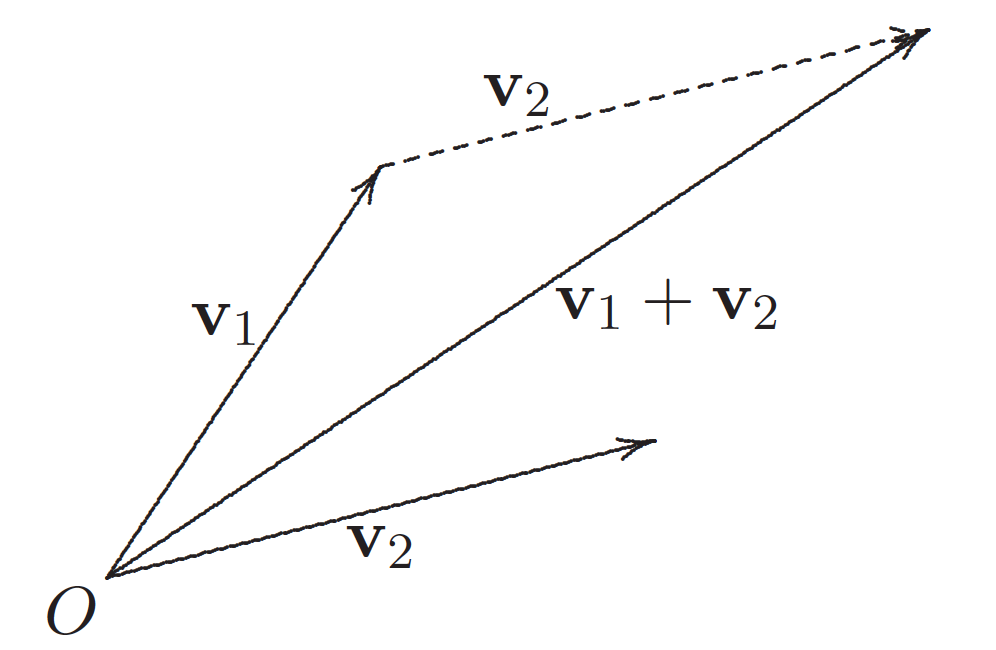
\includegraphics[width=\linewidth/3]{figures/fig4.png}
    \label{fig:4}
    \caption{Addition of two vectors}
  \end{figure}
\end{center}

The following exercise is for curious readers.

\begin{exercise}
  The set of all position vectors in $\R^3$ forms a normed vector space over $R$ with norm $| \dot |$. 
  (Please see the definition of vector space and normed vector space)
\end{exercise}

However, proving the next propositions are exercises for all readers because it is important to
understand and internalize the behavior of our Euclidean 3-space.

\begin{proposition}[Properties of vectors]
  Let $\pmb{a}, \pmb{b}, \pmb{c} \in \R^3$ and $\alpha, \beta \in \R$ then
  \begin{enumerate}
    \item $\pmb{a} + \pmb{b} = \pmb{b} + \pmb{a}$
    \item $\pmb{a} + (\pmb{b} + \pmb{c}) = (\pmb{a} + \pmb{b}) + \pmb{c}$
    \item $\pmb{a} + \pmb{0} = \pmb{a}$
    \item $\pmb{a} + \pmb{-a} = \pmb{0}$
    \item $\alpha(\pmb{a} + \pmb{b}) = \alpha \pmb{a} + \alpha \pmb{b}$
    \item $\alpha \pmb{a} = \pmb{a} \alpha$
    \item $(\alpha + \beta) \pmb{a} = \alpha \pmb{a} + \beta \pmb{a}$
    \item $(\alpha\beta)\pmb{a} = \alpha(\beta \pmb{a})$
    \item $1\pmb{a} = \pmb{a}$
    \item $|\alpha \pmb{a}| = |\alpha| | \pmb{a} |$
  \end{enumerate}
\end{proposition}

\begin{exercise}
  Prove the Proposition 2.1 .
\end{exercise}

\begin{proposition}
  Prove the triangle inequality $|v_1 + v_2| \leq |v_1| + |v_2|$ for all $v_1, v_2 \in \R^3$.
\end{proposition}

\begin{exercise}
  Prove the Proposition 2.2 .
\end{exercise}

\subsection{Dot Product}

Until now, we have discussed only the multiplication of a vector and a scalar. However,
we can also define the multiplication of two vectors. A natural way to define a kind of vector product
is following.

\begin{defn}[Dot Product]
  Let $\pmb{a}, \pmb{b}$ be two vectors in $\R^3$. The dot product (or sometimes called scalar product)
  of $\pmb{a}$ and $\pmb{b}$ is the number $a \cdot b = a_1b_1 + a_2b_2 + a_3b_3$. It is 
  sometimes denoted by $\langle \pmb{a}, \pmb{b}\rangle$.
\end{defn}

\begin{example}
  Let $\pmb{a} = (1,2,3)$ and $\pmb{b} = (-1, 0, -1)$. Then we can compute dot product of these vectors as
  $$ \pmb{a} \cdot \pmb{b} = (1)(-1) + (2)(0) + (3)(-1) = -4 .$$
\end{example}

We can state the properties of the dot product as the following proposition.

\begin{proposition}[Properties of the Dot Product]
  Let $\pmb{a},\pmb{b}, \pmb{c} \in \R^3$, then
  \begin{enumerate}
    \item $\pmb{a} \cdot \pmb{a} = |\pmb{a}|^2$
    \item $\pmb{a} \cdot \pmb{b} = \pmb{b} \cdot \pmb{a}$
    \item $\pmb{a} \cdot (\pmb{b} + \pmb{c}) = \pmb{a} \cdot \pmb{b} + \pmb{a} \cdot \pmb{c}$
    \item $(\alpha \pmb{a}) \cdot \pmb{b} = \alpha(\pmb{a} \cdot \pmb{b}) = \pmb{a} \cdot (\alpha \pmb{b})$
    \item $\pmb{0} \cdot \pmb{a} = \pmb{0}$
  \end{enumerate}
\end{proposition}

\begin{exercise}
  Prove the Proposition 2.3 .
\end{exercise}

Following exercise and theorem are for REALLY curious students.
\begin{proposition}
  Let $\pmb{a}$ be a vector in $\R^3$. Then define the function 
  $f:\R^3 \rightarrow \R$ as
  $f(\pmb{x}) = \pmb{x} \cdot \pmb{a}$. Then $f$ is linear(what?).
\end{proposition}
\begin{exercise}
  Prove the Proposition 2.4 .
\end{exercise}

Okay! It was not that surprising. What about the next statement?
\begin{thm}[Riesz representation theorem]
  Let $f: \R^3 \rightarrow \R$ be any linear (what?) and continuous (what?) function. Then,
  there exists a unique $\pmb{v} \in \R^3$ such that 
  $$ f(\pmb{x}) = \pmb{x} \cdot \pmb{v} $$
\end{thm}

Now we can continue to our main discussion and obtain the main result of this section.

\begin{thm}
  If $\theta$ is the angle between the vectors $\pmb{a}$ and $\pmb{b}$, then
  $$ \pmb{a} \cdot \pmb{b} = |\pmb{a}| \cdot |\pmb{b}| \cos \theta, \quad 0 \leq \theta \leq \pi.$$
\end{thm}

\begin{proof}
  Let $\pmb{OA}=\pmb{a}$ and $\pmb{OB}=\pmb{b}$, where $O$ is the origin and $\theta = \angle AOB$.
  
  \begin{center}
    \begin{figure}[h]
      \centering
      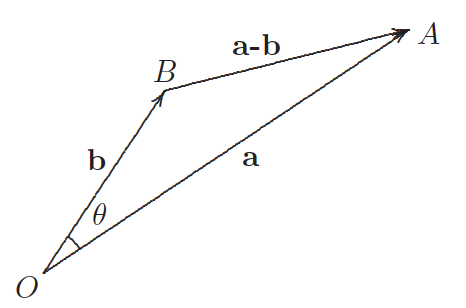
\includegraphics[width=\linewidth/3]{figures/fig5.png}
      \label{fig:5}
      \caption{Vector subtraction}
    \end{figure}
  \end{center}

  Applying cosine rule to $\triangle OAB$, we have
  $$ |\pmb{a} - \pmb{b}|^2 = |\pmb{a}|^2 + |\pmb{b}|^2 - 2 |\pmb{a}| \cdot |\pmb{b}| \cos \theta $$
  Also, we know from the properties of the dot product that (why?)
  $$ |\pmb{a} - \pmb{b}|^2 = (\pmb{a} - \pmb{b}) \cdot (\pmb{a} - \pmb{b}) = |\pmb{a}|^2 + |\pmb{b}|^2 - 2 \pmb{a} \cdot \pmb{b}$$
  Therefore, $ \pmb{a} \cdot \pmb{b} = |\pmb{a}| \cdot |\pmb{b}| \cos \theta $ or
  $$ \cos \theta = \frac{\pmb{a} \cdot \pmb{b}}{ |\pmb{a}| \cdot |\pmb{b}|} $$
\end{proof}

Two vectors $\pmb{a}$ and $\pmb{b}$ are said to be orhogonal or perpendicular if the angle between them is $90^\circ$.
In other words,
$$ \pmb{a} \text{ and } \pmb{b} \text{ are orthogonal} \iff \pmb{a} \cdot \pmb{b} = 0 \text{ (why?)}$$.

Now based on this theorem, we will discuss the projection of a vector along another vector.
Let $\pmb{a}$ and $\pmb{b}$ be two vectors in $\R^3$. Let's represent $\pmb{a}$ as 
$\pmb{PQ}$ and $\pmb{b}$ as $\pmb{PR}$.

\begin{center}
  \begin{figure}[h]
    \centering
    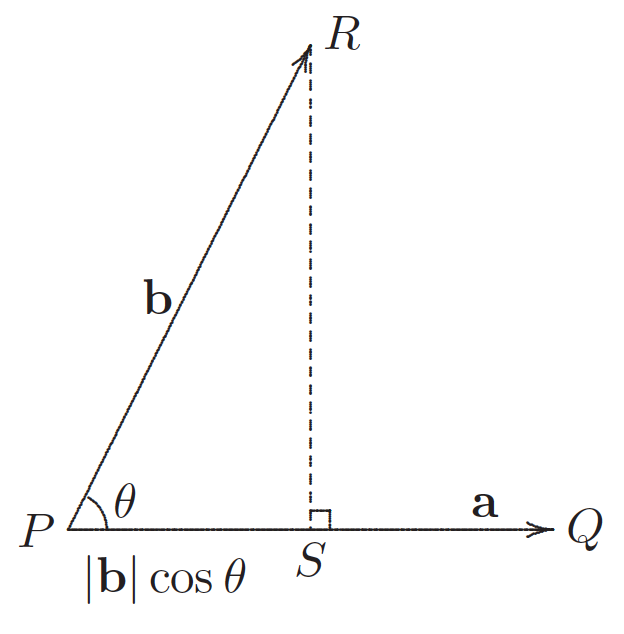
\includegraphics[width=\linewidth/4]{figures/fig6.png}
    \label{fig:6}
    \caption{Projection of a vector to another one}
  \end{figure}
\end{center}

Then
$$ |\pmb{b}| \cos \theta = \frac{\pmb{a} \cdot \pmb{b}}{| \pmb{a} |} = \frac{\pmb{a}}{|\pmb{a}|} \cdot \pmb{b} .$$

\begin{defn}
  \begin{enumerate} Let $\pmb{a}$ and $\pmb{b}$ be two vectors in $\R^3$.
    \item The scalar projection of $\pmb{b}$ onto $\pmb{a}$ is $|\pmb{b}|\cos \theta = \frac{\pmb{a}}{|\pmb{a}|} \cdot \pmb{b}$.
    \item The vector projection of $\pmb{b}$ onto $\pmb{a}$ is 
    $ \left( \frac{\pmb{a}}{ |\pmb{a}| } \cdot \pmb{b} \right) \frac{\pmb{a}}{|\pmb{a}|} 
     = \frac{ \pmb{a} \cdot \pmb{b} }{|\pmb{a}|^2}\pmb{a}$.
  \end{enumerate}
\end{defn}

Note that the scalar projection is negative if $\theta > 90^\circ$. Moreover, 
$\pmb{SR}=\pmb{PR}-\pmb{PS}=\pmb{b} - \frac{ \pmb{a} \cdot \pmb{b} }{|\pmb{a}|^2}\pmb{a}$.
Thus the distance from $R$ to the line $PQ$ is given by
$$ |\pmb{RS}| = \left| \pmb{b} - \frac{ \pmb{a} \cdot \pmb{b} }{|\pmb{a}|^2}\pmb{a} \right| $$ 

\begin{exercise}
  Prove the Cauchy-Schwarz inequality: $|\pmb{a} \cdot \pmb{b}| \leq |\pmb{a}| |\pmb{b}|$. Also, determine when the equality holds.
\end{exercise}

\subsection{The Cross Product}
\begin{defn}
  Let $\pmb{a}, \pmb{b} \in \R^3$, then the cross product (or sometimes called vector product)
  of $\pmb{a}$ and $\pmb{b}$ is 
  \begin{align*}
    \pmb{a} \times \pmb{b} &= (a_2b_3 - a_3b_2, a_3b_1 - a_1b_3, a_1b_2 - a_2b_1) \\
        &=  
        \begin{vmatrix}
          \pmb{i} & \pmb{j} & \pmb{k} \\
          a_1 & a_2 & a_3 \\
          b_1 & b_2 & b_3
        \end{vmatrix} \\
        &= 
        \begin{vmatrix}
          a_2 & a_3 \\
          b_2 & b_3 \\
        \end{vmatrix} \pmb{i}
        - \begin{vmatrix}
          a_1 & a_3 \\
          b_1 & b_3 \\
        \end{vmatrix} \pmb{j}
        + \begin{vmatrix}
          a_1 & a_2 \\
          b_1 & b_2 \\
        \end{vmatrix} \pmb{k}
  \end{align*}
\end{defn}

\begin{exercise}
  Let $\pmb{a} = (1,3,4)$ and $\pmb{b} = (2,7,-5)$. Find $\pmb{a} \times \pmb{b}$.
\end{exercise}

\begin{thm}
  Let $\pmb{a}, \pmb{b}, \pmb{c} \in \R^3$. Then 
  \[
    \pmb{a} \cdot (\pmb{b} \times \pmb{c}) =  
    \begin{vmatrix}
      a_1 & a_2 & a_3 \\
      b_1 & b_2 & b_3 \\
      c_1 & c_2 & c_3
    \end{vmatrix}
  \]
\end{thm}

\begin{exercise}
  Prove the Theorem 2.3 .
\end{exercise}

\begin{corollary}
  $\pmb{b} \times \pmb{c}$ is perpendicular to both $\pmb{b}$ and $\pmb{c}$.
\end{corollary}

\begin{proof}
  Use previous theorem and singularity(what?) of the matrix and conclude that the determinant is $0$.
\end{proof}

Next result is the main result of this section.

\begin{thm}
  If $\theta$ is the angle between $\pmb{a}$ and $\pmb{b}$, $0\leq \theta \leq \pi$, then $|\pmb{a} \times \pmb{b}| = |\pmb{a}||\pmb{b}| \sin \theta$.
\end{thm}
\begin{proof}
  First we need the following identity
  $$(a_2b_3-a_3b_2)^2+(a_3b_1-a_1b_3)^2+(a_1b_2-a_2b_1)^2=(a_1^2+a_2^2+a^2_3)(b_2^1+b_2^2+b_2^3)-(a_1b_1+a_2b_2+a_3b_3)^2$$
  which can be easily verified by direct simplification of both sides.
  Using this identity, we have
  
  \begin{align*}
    |\pmb{a} \times \pmb{b}|^2 &= (a_2b_3-a_3b_2)^2+(a_3b_1-a_1b_3)^2+(a_1b_2-a_2b_1)^2 \\
      &= (a_1^2+a_2^2+a^2_3)(b_2^1+b_2^2+b_2^3)-(a_1b_1+a_2b_2+a_3b_3)^2 \\
      &= |\pmb{a}|^2|\pmb{b}|^2 - (\pmb{a} - \pmb{b})^2 \\
      &= |\pmb{a}|^2|\pmb{b}|^2 - |\pmb{a}|^2|\pmb{b}|^2\cos^2 \theta \\
      &= |\pmb{a}|^2|\pmb{b}|^2\sin^2 \theta
  \end{align*}

  Since $0 \leq \theta \leq \pi$, $\sin \geq 0$, we have $|\pmb{a} \times \pmb{b}| = |\pmb{a}||\pmb{b}|\sin \theta$.
\end{proof}

It follows from this result that $|\pmb{a} \times \pmb{b}| = |\pmb{a}||\pmb{b}|\sin \theta$ 
is the area of the parallelogram determined by $a$ and $b$.

\begin{center}
  \begin{figure}[h]
    \centering
    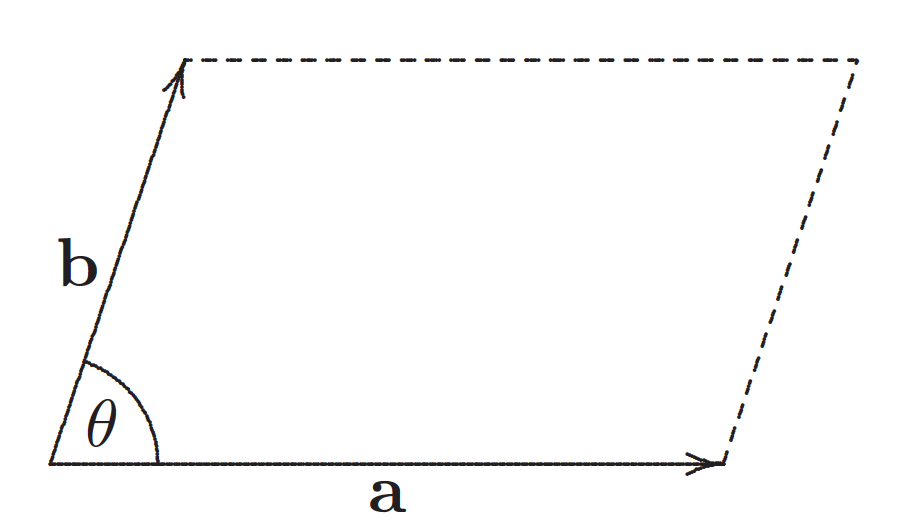
\includegraphics[width=\linewidth/3]{figures/fig7.png}
    \label{fig:7}
    \caption{Parallelogram lying between two vectors}
  \end{figure}
\end{center}

$\pmb{a} \times \pmb{b}$ is a vector perpendicular to the plane spanned by $\pmb{a}$ and $\pmb{b}$ with magnitude 
$|\pmb{a}||\pmb{b}|\sin \theta$, where $0 \leq \theta \leq \pi$ is the angle between $\pmb{a}$ and $\pmb{b}$.

\begin{center}
  \begin{figure}[h]
    \centering
    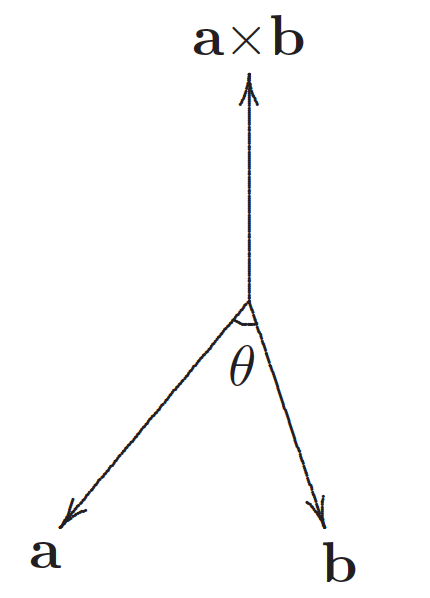
\includegraphics[width=\linewidth/5]{figures/fig8.png}
    \label{fig:8}
    \caption{Cross product of two vectors in $R^3$}
  \end{figure}
\end{center}

There are two possible choices of such a vector. The choice is determined by the right-hand
rule: $\pmb{a}\times\pmb{b}$ is directed so that a right-hand rotation about $\pmb{a} \times \pmb{b}$ through an angle $\theta$ 
will carry $\pmb{a}$ to the direction of $\pmb{b}$.

\begin{proposition}[Properties of the Cross Product]
  Let $\pmb{a}, \pmb{b}, \pmb{c}$ be three vectors in $\R^3$ and $\alpha \in \R$.
  \begin{enumerate}
    \item $\pmb{a} \times \pmb{b} = - \pmb{b} \times \pmb{a}$
    \item $(\alpha\pmb{a}) \times \pmb{b} = \alpha(\pmb{a} \times \pmb{b}) = \pmb{a} \times (\alpha \pmb{b})$
    \item $\pmb{a} \times (\pmb{b} + \pmb{c}) = \pmb{a} \times \pmb{b} + \pmb{a} \times \pmb{c}$
    \item $(\pmb{a} + \pmb{b}) \times \pmb{c} = \pmb{a} \times \pmb{c} + \pmb{b} \times \pmb{c}$
    \item $\pmb{a} \cdot (\pmb{b} \times \pmb{c}) = (\pmb{a} \times \pmb{b}) \cdot \pmb{c}$
    \item $\pmb{a} \times (\pmb{b} \times \pmb{c}) = (\pmb{a} \cdot \pmb{c})\pmb{b} - (\pmb{a} \cdot \pmb{b}) \pmb{c}$
  \end{enumerate}
\end{proposition}

\begin{exercise}
  Prove the Proposition 2.5 .
\end{exercise}

\section{Area Calculation}
\subsection{Area of Triangle}
We already saw that the cross product of two vectors gives us the area of the 
parallelogram determined by those vectors. Dividing that quantity by $2$ will give us the 
area of the triangle that lies between those vectors.

As we discussed earlier, we know that the cross product of two vectors can be positive or negative.
We also learned that this sign can be determined by the right-hand rule. 
Now let's see how we can use this property of cross product in $\R^2$ to determine the positions of two vectors in comparison to each other or relation between the orientation of the points.

Let $\pmb{v}$ and $\pmb{v}$ be two vectors in $\R^2$. Then putting the definition of cross product will give us

\[
\pmb{u} \times \pmb{v} =  
\begin{vmatrix}
  u_2 & u_3 \\
  v_2 & v_3 \\
\end{vmatrix} \pmb{i}
- \begin{vmatrix}
  u_1 & u_3 \\
  v_1 & v_3 \\
\end{vmatrix} \pmb{j}
+ \begin{vmatrix}
  u_1 & u_2 \\
  v_1 & v_2 \\
\end{vmatrix} \pmb{k}
\]

Since $u_3=v_3=0$, first two determinant values will be zero and the cross product
will have only $\pmb{k}$ component. Now, let's denote the $\pmb{k}$ component of 
that cross product as $(\pmb{u} \times \pmb{v})_k$. Then,

\[ 
(\pmb{u} \times \pmb{v})_k =   
\begin{cases} 
  negative & \text{if $v$ lies in left hand side of the $u$} \\
  0 & \text{if $u$ and $v$ lies in the same line} \\
  positive & \text{if $v$ lies in right hand side of the $u$}
\end{cases}
\]

Then we can also interpret this result for determining the orientation of three ordered
points in $\R^2$. Let $P,Q,R$ be points in $\R^2$ then

\[ 
(\pmb{PQ} \times \pmb{PR})_k =   
\begin{cases} 
  negative & \text{if $\pmb{PR}$ lies in left hand side of the $\pmb{PQ}$} \\
  0 & \text{if $\pmb{PQ}$ and $\pmb{PR}$ lies in the same line} \\
  positive & \text{if $\pmb{PR}$ lies in right hand side of the $\pmb{PQ}$}
\end{cases}
\]

or equivalently

\[ 
(\pmb{PQ} \times \pmb{PR})_k =   
\begin{cases} 
  negative & \text{P,Q and R in counter-clockwise order}\\
  0 & \text{P,Q and R lies in the same line} \\
  positive & \text{P,Q and R in clockwise order}
\end{cases}
\]

We already discussed that $\frac{|\pmb{PQ} \times \pmb{PR}|}{2} = \frac{|(\pmb{PQ} \times \pmb{PR})_k|}{2} = |A(\triangle PQR)|$ and now,
we will define the $A(\triangle PQR) := \frac{(\pmb{PQ} \times \pmb{PR})_k}{2}$ as the signed area of the triangle (see that it is scalar).
While the sign is positive if the points are in counter-clockwise order, it is negative if the points are in clockwise order.

\lstset{language=C++,
                basicstyle=\ttfamily,
                keywordstyle=\color{blue}\ttfamily,
                stringstyle=\color{red}\ttfamily,
                commentstyle=\color{gray}\ttfamily,
                morecomment=[l][\color{magenta}]{\#}
}

The following implementation is taken from [4].
\begin{lstlisting}
    // Assume Point is a class with two properties of double x and y
    inline double signedTriangleArea( Point P0, Point P1, Point P2 )
    {
        return ( (P1.x - P0.x) * (P2.y - P0.y)
               - (P2.x - P0.x) * (P1.y - P0.y) )/2;
    }
\end{lstlisting}

\subsection{Area of a Simple Polygon}
Based on a signed area of the triangle we will build our area calculation algorithm of any simple polygon (i.e. ones without self-intersection).

Let $\Omega$ be a simple polygon in $\R^2$ whose vertices are defined by $V_i = (x_i, y_i)$
for $i = 0,1 \cdots n$, and define $V_0 = V_n$ and let $P$ be any point. 
For each edge from $V_i$ to $V_{i+1}$ of $\Omega$ $\triangle_i = \triangle PV_iV_{i+1}$ where
$i = 0,1, \cdots n_1$ forms a triangle. Now we can calculate the signed area of the polygon $\Omega$
by the following equation
$$ A(\Omega) = \sum_{i=0}^{n-1} A(\triangle_i) \text{ where } \triangle_i = \triangle PV_iV_{i+1}$$

Notice that for a counterclockwise oriented polygon, when the point $P$ is on 
the "inside" left side of an edge $\pmb{V_iV_{i+1}}$, the area of $\triangle_i$ is positive; 
whereas, when $P$ is on the "outside" right side of an edge $\pmb{V_iV_{i+1}}$,  $\triangle_i$
has a negative area. If instead the polygon is oriented clockwise, then the 
signs are reversed, and inside triangles become negative.

\begin{center}
  \begin{figure}[h]
    \centering
    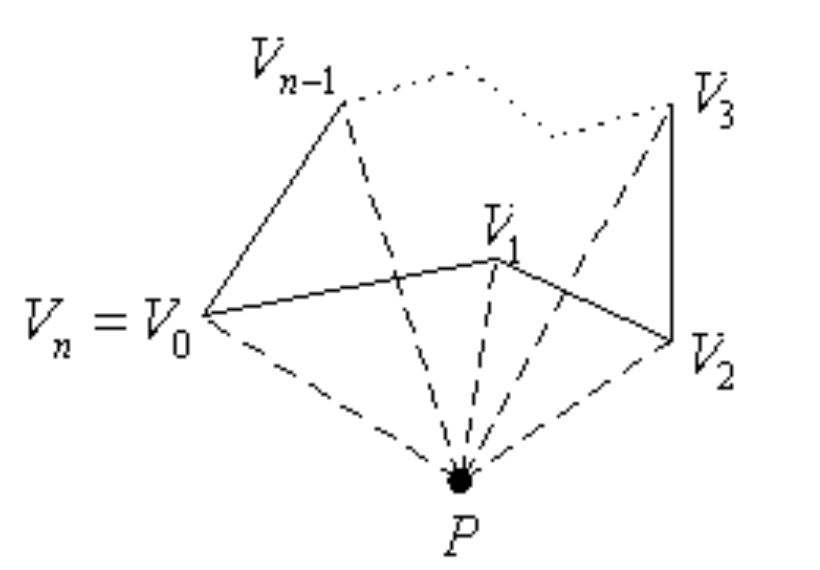
\includegraphics[width=\linewidth/2]{figures/fig26.png}
    \label{fig:8}
    \caption{Illustration of polygon area calculation.}
  \end{figure}
\end{center}

For example, in the Figure 9, the triangles $\triangle_2$ and $\triangle_{n-1}$ have 
positive area, and contribute positively to the total area of polygon $\Omega$. 
However, as one can see, only part of $\triangle_2$ and $\triangle_{n-1}$ are actually inside 
$\Omega$ and there is a part of each triangle that is also exterior. 
On the other hand, the triangles $\triangle_0$ and $\triangle_1$ have negative area, and 
this cancels out the exterior excesses of positive area triangles. 
In the final analysis, the exterior areas all get canceled, and one is left with 
exactly the area of the polygon $\Omega$.

One can make the formula more explicit by picking a specific point $P$ and 
expanding the terms. By selecting $P=(0,0)$, the area formula of each triangle 
reduces to $2A(\triangle_i)=(x_iy_{i+1}-x_{i+1}y_i)$. This yields:

\begin{align*}
  2A(\Omega) &= \sum_{i=0}^{n-1} (x_iy_{i+1} - x_{i+1}y_i) \\
  &= \sum_{i=0}^{n-1} (x_i + x_{i+1})(y_{i+1} - y_i) \\
  &= \sum_{i=0}^{n} x_i(y_{i+1} - y_i)
\end{align*}

where $V_i = (x_i, y_i)$, with $i(mod\ n)$. (Think about the equations given above!).

The following implementation is taken from [4].
\begin{lstlisting}
// area2D_Polygon(): compute the area of a 2D polygon
//  Input:  int n = the number of vertices in the polygon
//          Point* V = an array of n+1 vertex points with V[n]=V[0]
//  Return: the (double) area of the polygon
double area2D_Polygon( int n, Point* V )
{
    double area = 0;
    int  i, j, k;   // indices

    if (n < 3) return 0;  // a degenerate polygon

    for (i=1, j=2, k=0; i<n; i++, j++, k++) {
        area += V[i].x * (V[j].y - V[k].y);
    }
    area += V[n].x * (V[1].y - V[n-1].y);  // wrap-around term
    return area / 2.0;
}
\end{lstlisting}

\section{Lines and Planes}
\subsection{Lines}
In space, we can represent lines in multiple ways. As you know, we can represent lines with linear equations. Although linear equations represent lines in 2D, the single linear equation represents a plane in 3D. In addition to linear equations, we can express lines with a point and direction vector.
Here is the summary of the expressions with their names and usage:

\begin{center}
  \begin{tabular}{ c c c }
   \underline{Type} & \underline{Equation} & \underline{Usage} \\
   Explicit 2D & $y=f(x)=mx+b$ & a non-vertical 2D line \\ 
   Implicit 2D & $f(x,y)=ax+by+c=0$ & any 2D line \\  
   Parametric & $P(t) = P_0+t\pmb{v_L}$ & any line in any dimension    
  \end{tabular}
\end{center}

The equivalence of these representations and the conversion between them can be derived easily.
However, for this course, we will use the parametric representation and we will discuss
distance calculations based on this type of expressions.

We already discussed that the cross product of two vectors gives us the area of the
parallelogram that lies between these two vectors. Now, we will use this notion
to derive a formula to calculate the distance between a point and a line.

Firstly we will discuss 2D case, let $P_0$ and $P_1$ be any two distinct points on a line $L$ and $P$ be any point
from which we want to calculate distance to line $L$. Now, set two vectors
$\pmb{v_L} = P_1-P_0$ and $\pmb{w}=P-P_0$. From section 2 we know that 
$\pmb{v_L} \times \pmb{w} = |\pmb{v_L}||\pmb{w}||\sin \theta|$ where 
$\theta$ is the angle between two vectors. This quantity also equals to the area of
the parallelogram lying between vectors. Dividing the area with the length of base will give us the distance between the point and the base line or formally.

$$ d(P,\pmb{L}) = \frac{|\pmb{v_L} \times \pmb{w}|}{|\pmb{v_L}|} = 
|\pmb{u_L} \times \pmb{w}| $$

where $\pmb{u_L} = \pmb{v_L}/|\pmb{v_L}|$. If one is computing the distances of many points to a 
fixed line, then it is most efficient to first calculate $\pmb{u_L}$.

\begin{exercise}
  Think about why this works only for 2D spaces.
\end{exercise}

For higher dimensions, we can calculate the distance using the projection. Suppose 
that we have the same setting as before. We can express our line as: 
$P(t):=P_0 + t(P_1-P_0)=P_0+t\pmb{v_L}$
Now, let's find the projection $P(b)$ of vector $\pmb{w} = \pmb{P_0P}$ 
to the vector $\pmb{v_L} = \pmb{P_0P_1}$.

$$
  b =\frac{d(P_0,P(b))}{d(P_0, P_1)} 
    =\frac{|\pmb{w}|\cos \theta}{\pmb{v_L}} 
    =\frac{\pmb{w}\cdot\pmb{v_L}}{|\pmb{v_L}|^2}
    =\frac{ \pmb{w}\cdot\pmb{v_L} }{ \pmb{v_L}\cdot\pmb{v_L} }
$$

and thus:

$$
d(P,\pmb{L}) = |P-P(b)| = |\pmb{w} - b\pmb{v_L}| = |\pmb{w} - (\pmb{w}\cdot\pmb{u_L})\pmb{u_L}|
$$

where $\pmb{u_L}$ denotes unit vector as defined above and $\theta$ denotes the angle between the vectors.

By using this notion we can find the distance between a point and a line segment.
Firstly let's discuss the concepts of rays and line segments. 
A \textbf{ray R} is a half line originating at a point P0 and extending 
indefinitely in some direction. It can be expressed parametrically as 
$P(t)$ for all $t \geq 0$ with $P(0) = P_0$ as the starting point.
A finite segment S consists of the points of a line that are between two 
endpoints $P_0$ and $P_1$. Again, it can be represented by a parametric equation 
with $P(0) = P_0$ and $P(1) = P_1$ as the endpoints and the points $P(t)$ for 
$0\leq t \leq 1$ as the segment points.

The thing that is different about computing distances of a point $P$ to a ray 
or a segment is that the base $P(b)$ of the perpendicular from $P$ to the extended 
line $\pmb{L}$ may be outside the range of the ray or segment. In this case, the actual 
shortest distance is from the point $P$ to the start point of the ray or one of 
the endpoints of a finite segment. The following figure illustrates the possible 
extreme conditions for the rays and line segments.

\begin{center}
  \begin{figure}[h]
    \centering
    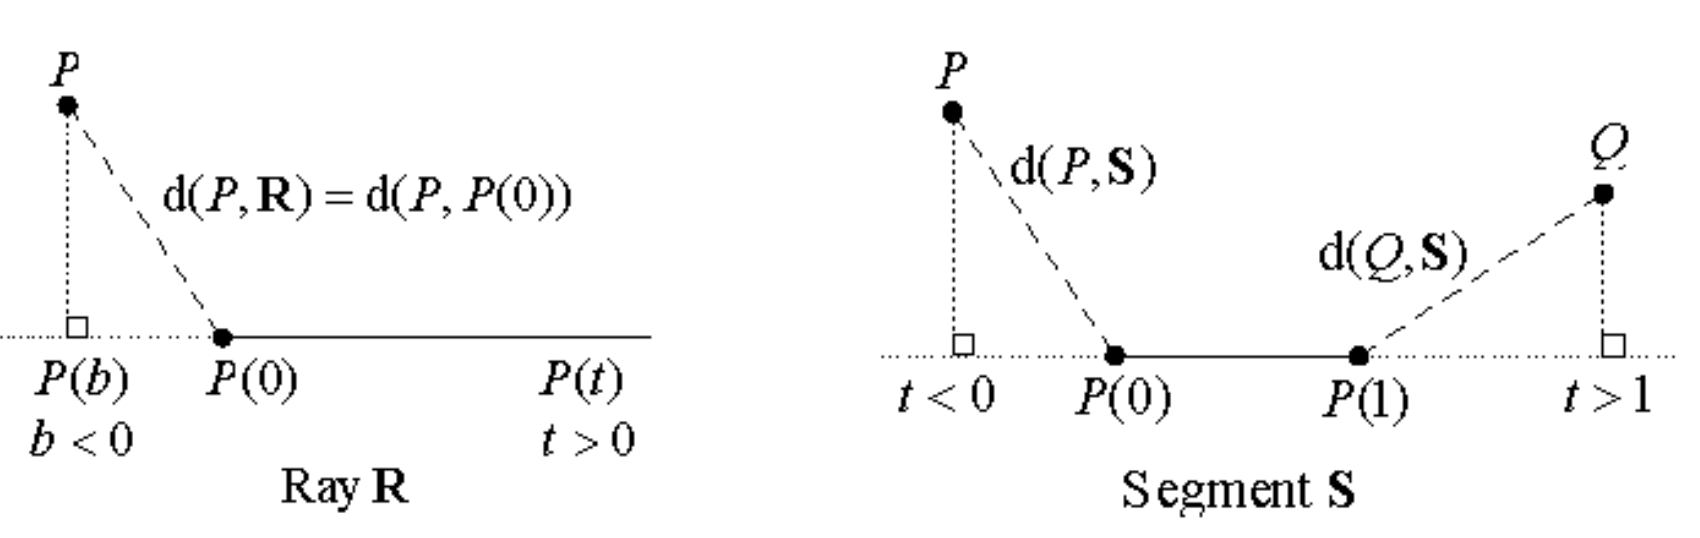
\includegraphics[width=.9\linewidth]{figures/fig9.png}
    \label{fig:9}
    \caption{Point-Ray and Point-Line Segment distance calculations}
  \end{figure}
\end{center}


In order to find the distance to a line segment, we will first calculate the value of
$b$ as above. Then, by checking that whether $P(b)$ lies on the line segment or not,
we will find the nearest point of the line segment to the point.

The following implementation is taken from [4].
\begin{lstlisting}
// Copyright 2001 softSurfer, 2012 Dan Sunday
// This code may be freely used, distributed and modified for any purpose
// providing that this copyright notice is included with it.
// SoftSurfer makes no warranty for this code, and cannot be held
// liable for any real or imagined damage resulting from its use.
// Users of this code must verify correctness for their application.
 

// Assume that classes are already given for the objects:
//     Point and Vector with
//          coordinates {float x, y, z;} (z=0  for 2D)
//          appropriate operators for:
//               Point  = Point ± Vector
//               Vector = Point - Point
//               Vector = Scalar * Vector
//     Line with defining endpoints {Point P0, P1;}
//     Segment with defining endpoints {Point P0, P1;}
//===================================================================

// dot product (3D) which allows vector operations in arguments
#define dot(u,v)   ((u).x * (v).x + (u).y * (v).y + (u).z * (v).z)
#define norm(v)     sqrt(dot(v,v))     // norm = length of  vector
#define d(u,v)      norm(u-v)          // distance = norm of difference


// dist_Point_to_Line(): get the distance of a point to a line
//     Input:  a Point P and a Line L (in any dimension)
//     Return: the shortest distance from P to L
float dist_Point_to_Line( Point P, Line L)
{
     Vector v = L.P1 - L.P0;
     Vector w = P - L.P0;

     double c1 = dot(w,v);
     double c2 = dot(v,v);
     double b = c1 / c2;

     Point Pb = L.P0 + b * v;
     return d(P, Pb);
}


// dist_Point_to_Segment(): get the distance of a point to a segment
//     Input:  a Point P and a Segment S (in any dimension)
//     Return: the shortest distance from P to S
float dist_Point_to_Segment( Point P, Segment S)
{
     Vector v = S.P1 - S.P0;
     Vector w = P - S.P0;

     double c1 = dot(w,v);
     if ( c1 <= 0 )
          return d(P, S.P0);

     double c2 = dot(v,v);
     if ( c2 <= c1 )
          return d(P, S.P1);

     double b = c1 / c2;
     Point Pb = S.P0 + b * v;
     return d(P, Pb);
}

\end{lstlisting}

\subsection{Planes}
In order to keep these notes as compact as possible we won't dive into the details
of the distance calculations between points and planes. However, a curious reader may consult to the excellent reference of [4] for distance calculations and 
their implementations.

\section{Intersection}
We discussed the parametric representation of lines in Section 4. 
In this section, we will deal with intersection points of lines and
line segments of 2D Euclidean space. However, for more details
about intersections in higher dimensions and intersections of 
higher dimensional surfaces (planes), one can consult the [4].

For the 2D case, we will examine two possible configurations separately.
We will work on parallel lines and then work on the non-parallel case.

\subsection{Parallel Lines}
Two lines are parallel if and only if their direction vectors are 
collinear, namely when the two vectors $\pmb{u}=\pmb{P_1-P_0}$ 
and $\pmb{v}=\pmb{Q_1-Q_0}$ are linearly related as 
$\pmb{u} = a\pmb{v}$ for some real number $a$.

When we discussed the properties of dot product, we already saw that
two vectors are perpendicular when their dot product is $0$. Now,
we will use this notion to check whether two vectors are co-linear
or not. Suppose that $\pmb{u} = (u_1, u_2)$, then a perpendicular 
vector $\pmb{u}^\perp$ can be defined as $\pmb{u}^\perp = (-u_2, u_1)$.
One can easily check that $\pmb{u} \cdot \pmb{u}^\perp = 0$.
Now, by considering the value of $\pmb{v} \cdot \pmb{u}^\perp$,
we can check whether two vectors are co-linear or not.

In order to check whether a point $P_0$ lies on a line $Q(t)$,
one can use simple linear calculations. If $P_0$ lies on the $Q(t)$
and $Q(t)$ is represented by a point $Q_0$ and direction vector
\pmb{v} as $Q(t) = Q_0 + t\pmb{v}$, we can write
$$ P_0 = Q_0 + t_0 \pmb{v} \text{ , for some } t_0$$
Then, we can use this notion to check our desire, let 
$\pmb{w}=\pmb{Q_0P_0}$ or $\pmb{w} = Q_0 - P_0$. Then if $P_0$
lies on $Q(t)$ then $\pmb{w}$ and $\pmb{v}$ must be co-linear, and
we can check this as we have discussed above. We can calculate 
the value of $t_0$ as $t_0 = \frac{w_0}{v_1}$.

If both lines are finite segments, then they may (or may not) 
overlap. In this case, solve for $t_0$ and $t_1$ such that $P_0 = Q(t_0)$ 
and $P_1 = Q(t_1)$. If the segment intervals $[t_0,t_1]$ and $[0,1]$ are 
disjoint, there is no intersection. Otherwise, intersect the 
intervals (using max and min operations) to get 
$[r_0,r_1]=[t_0,t_1] \cap [0,1]$. Then the intersection segment is 
$\pmb{Q(r_0)Q(r_1)}=\pmb{P_0P_1} \cap \pmb{Q_0Q_1}$. This works in any dimension.

\subsection{Non-parallel Lines}
When the two lines or segments are not parallel, they might 
intersect in a unique point. In 2D Euclidean space, infinite 
lines always intersect. In higher dimensions, they usually miss 
each other and do not intersect. But if they intersect, then 
their linear projections onto a 2D plane will also intersect. 
So, one can simply restrict situation to two coordinates, for which $\pmb{u}$ and $\pmb{v}$ (direction vectors)
are not parallel, compute the 2D intersection point $I$ at $P(s_I)$
and $Q(t_I)$ for those two coordinates, and then test if 
$P(s_I) = Q(t_I)$ for all coordinates. To compute the 2D 
intersection point, consider the two lines and the associated 
vectors in the diagram:

\begin{center}
  \begin{figure}[!htb]
    \centering
    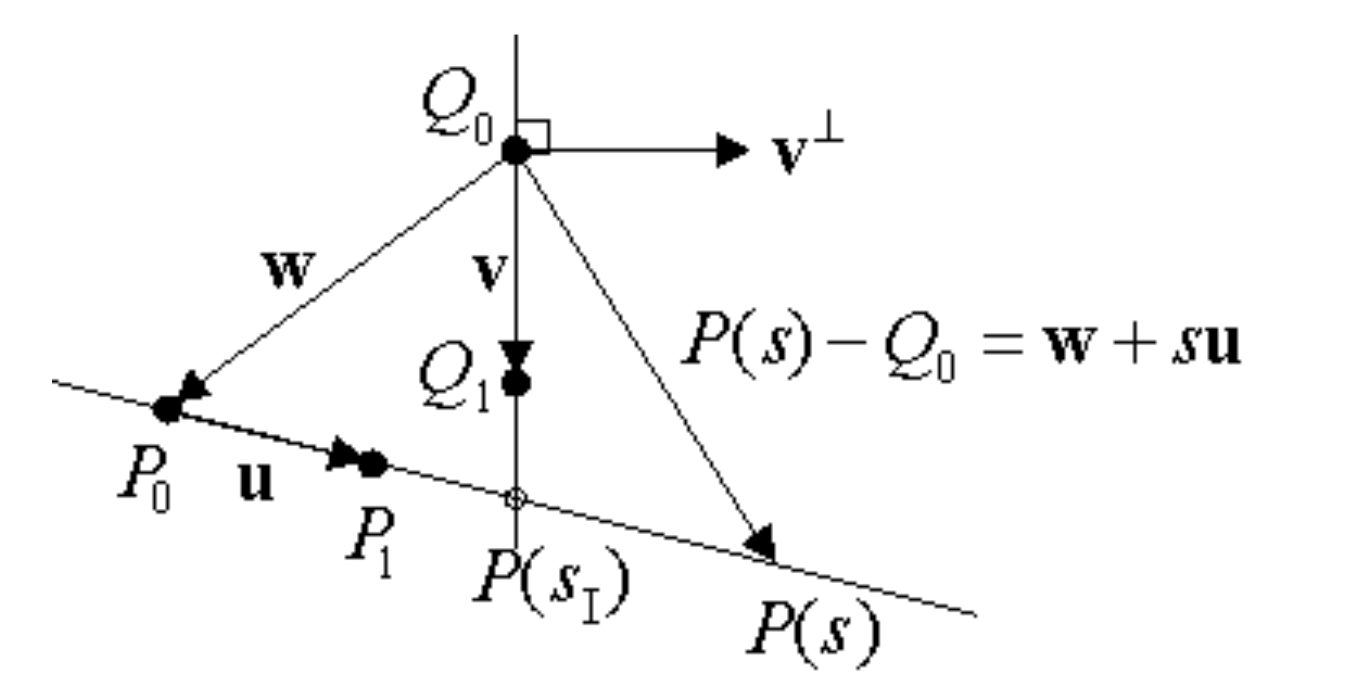
\includegraphics[width=.5\linewidth]{figures/fig18.png}
    \label{fig:10}
    \caption{Illustration of finding intersection of two lines}
  \end{figure}
\end{center}

To determine $s_I$, we have the vector equality $P(s)-Q_0=\pmb{w}+s\pmb{u}$ where 
$\pmb{w}=P_0-Q_0$. At the intersection, the vector $P(s_I)-Q_0$ is perpendicular 
to $\pmb{v}^\perp$, and this is equivalent to the perp product condition 
that $\pmb{v}^\perp \cdot (\pmb{w}+s\pmb{u})=0$. Solving this equation, we get:

\[ 
  s_I = \frac{-\pmb{v}^\perp \cdot \pmb{w}}{\pmb{v}^\perp \cdot \pmb{u}} 
      =  \frac{v_2w_1 - w_1v_2}{v_1u_2 - v_2u_1}
\]

Note that the denominator $\pmb{v}^\perp \cdot \pmb{u}=0$ only when the lines are parallel 
as previously discussed. Similarly, solving for $Q(t_I)$, we get:

\[
  t_I = \frac{\pmb{u}^\perp \cdot \pmb{w}}{\pmb{u}^\perp \cdot \pmb{v}} 
  = \frac{u_1w_2 - u_2w_1}{u_1v_2 - u_2v_1}  
\]

The denominators are the same up to sign, since 
$\pmb{u}^\perp \cdot \pmb{v}=-\pmb{v}^\perp \cdot \pmb{u}=0$, 
and should only be computed once if we want to know both $s_I$ and $t_I$. 
However, knowing either is enough to get the intersection point 
$I = P(s_I) = Q(t_I)$.

Further, if one of the two lines is a finite segment (or a ray), 
say $P_0P_1$, then the intersect point is in the segment only when 
$0\leq s_I \leq 1$ (or $s_I \geq 0$ for a ray). If both lines are segments, 
then both solution parameters, $s_I$ and $t_I$, must be in the $[0,1]$ 
interval for the segments to intersect. Although this sounds simple 
enough, the code for the intersection of two segments is a bit 
delicate since many special cases need to be checked (see the following implementation).


The following implementation is taken from [4].
\begin{lstlisting}
// Copyright 2001 softSurfer, 2012 Dan Sunday
// This code may be freely used and modified for any purpose
// providing that this copyright notice is included with it.
// SoftSurfer makes no warranty for this code, and cannot be held
// liable for any real or imagined damage resulting from its use.
// Users of this code must verify correctness for their application.
 

// Assume that classes are already given for the objects:
//    Point and Vector with
//        coordinates {float x, y, z;}
//        operators for:
//            == to test  equality
//            != to test  inequality
//            Point   = Point ± Vector
//            Vector =  Point - Point
//            Vector =  Scalar * Vector    (scalar product)
//            Vector =  Vector * Vector    (3D cross product)
//    Line and Ray and Segment with defining  points {Point P0, P1;}
//        (a Line is infinite, Rays and  Segments start at P0)
//        (a Ray extends beyond P1, but a  Segment ends at P1)
//    Plane with a point and a normal {Point V0; Vector  n;}
//===================================================================
 

#define SMALL_NUM   0.00000001 // anything that avoids division overflow
// dot product (3D) which allows vector operations in arguments
#define dot(u,v)   ((u).x * (v).x + (u).y * (v).y + (u).z * (v).z)
#define perp(u,v)  ((u).x * (v).y - (u).y * (v).x)  // perp product  (2D)

// intersect2D_2Segments(): find the 2D intersection of 2 finite segments
//    Input:  two finite segments S1 and S2
//    Output: *I0 = intersect point (when it exists)
//            *I1 =  endpoint of intersect segment [I0,I1] (when it exists)
//    Return: 0=disjoint (no intersect)
//            1=intersect  in unique point I0
//            2=overlap  in segment from I0 to I1
int intersect2D_2Segments( Segment S1, Segment S2, Point* I0, Point* I1 )
{
    Vector    u = S1.P1 - S1.P0;
    Vector    v = S2.P1 - S2.P0;
    Vector    w = S1.P0 - S2.P0;
    float     D = perp(u,v);

    // test if  they are parallel (includes either being a point)
    if (fabs(D) < SMALL_NUM) {           // S1 and S2 are parallel
        if (perp(u,w) != 0 || perp(v,w) != 0)  {
            return 0;                    // they are NOT collinear
        }
        // they are co-linear or degenerate
        // check if they are degenerate  points
        float du = dot(u,u);
        float dv = dot(v,v);
        if (du==0 && dv==0) {            // both segments are points
            if (S1.P0 !=  S2.P0)         // they are distinct  points
                 return 0;
            *I0 = S1.P0;                 // they are the same point
            return 1;
        }
        if (du==0) {                     // S1 is a single point
            if  (inSegment(S1.P0, S2) == 0)  // but is not in S2
                 return 0;
            *I0 = S1.P0;
            return 1;
        }
        if (dv==0) {                     // S2 a single point
            if  (inSegment(S2.P0, S1) == 0)  // but is not in S1
                 return 0;
            *I0 = S2.P0;
            return 1;
        }
        // they are co-linear segments - get  overlap (or not)
        float t0, t1;                    // endpoints of S1 in eqn for S2
        Vector w2 = S1.P1 - S2.P0;
        if (v.x != 0) {
                 t0 = w.x / v.x;
                 t1 = w2.x / v.x;
        }
        else {
                 t0 = w.y / v.y;
                 t1 = w2.y / v.y;
        }
        if (t0 > t1) {                   // must have t0 smaller than t1
                 float t=t0; t0=t1; t1=t;    // swap if not
        }
        if (t0 > 1 || t1 < 0) {
            return 0;      // NO overlap
        }
        t0 = t0<0? 0 : t0;               // clip to min 0
        t1 = t1>1? 1 : t1;               // clip to max 1
        if (t0 == t1) {                  // intersect is a point
            *I0 = S2.P0 +  t0 * v;
            return 1;
        }

        // they overlap in a valid subsegment
        *I0 = S2.P0 + t0 * v;
        *I1 = S2.P0 + t1 * v;
        return 2;
    }

    // the segments are skew and may intersect in a point
    // get the intersect parameter for S1
    float sI = perp(v,w) / D;
    if (sI < 0 || sI > 1)                // no intersect with S1
        return 0;

    // get the intersect parameter for S2
    float     tI = perp(u,w) / D;
    if (tI < 0 || tI > 1)                // no intersect with S2
        return 0;

    *I0 = S1.P0 + sI * u;                // compute S1 intersect point
    return 1;
}

// inSegment(): determine if a point is inside a segment
//    Input:  a point P, and a collinear segment S
//    Return: 1 = P is inside S
//            0 = P is  not inside S
int inSegment( Point P, Segment S)
{
    if (S.P0.x != S.P1.x) {    // S is not  vertical
        if (S.P0.x <= P.x && P.x <= S.P1.x)
            return 1;
        if (S.P0.x >= P.x && P.x >= S.P1.x)
            return 1;
    }
    else {    // S is vertical, so test y  coordinate
        if (S.P0.y <= P.y && P.y <= S.P1.y)
            return 1;
        if (S.P0.y >= P.y && P.y >= S.P1.y)
            return 1;
    }
    return 0;
}
\end{lstlisting}

\subsection{Further Readings}
If you are curious about intersections of types line-plane, plane-plane, 
more than $2$ planes, triangle-plane and triangle-triangle, then you should 
definitely take a look at [4]. 

\section{Inclusion Problem}
Inclusion problem is defined as determining the inclusion of a point $P$ in a 2D 
simple polygon. For this problem there are two common methods. These methods
actually work for non-simple planar polygons as well. 
\subsection{The Crossing Number Method}

This method counts the number of times a ray starting from a point P crosses a 
polygon boundary edge separating its inside and outside. If this number is even, 
then the point is outside; when the crossing number is odd, the point 
is inside. This is easy to understand intuitively. Each time the ray crosses a 
polygon edge, its in-out parity changes (since a boundary always separates inside 
from outside, why?). Eventually, any ray must end up beyond and outside the 
bounded polygon. So, if the point is inside, the sequence of crossings 
must be: in > out > ... > in > out, and there is an odd number of them. 
Similarly, if the point is outside, there are an even number of crossings in 
the sequence: out > in > ... > in > out.

\begin{figure}[h]
  \centering
  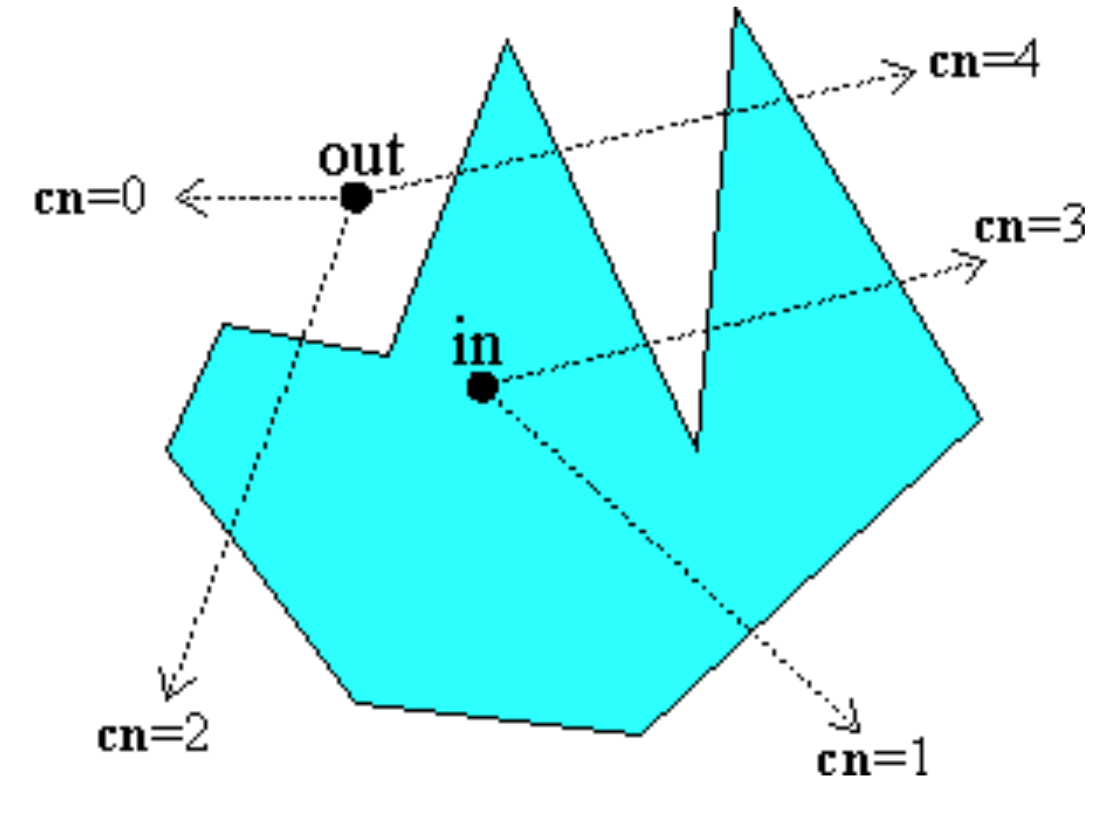
\includegraphics[width=.5\linewidth]{figures/fig10.png}
  \label{fig:11}
  \caption{Illustration of crossing number method}
\end{figure}

In implementing an algorithm for the crossing number method, one must ensure that only 
crossings that change the in-out parity are counted. In particular, special 
cases where the ray passes through a vertex must be handled properly. These 
include the following types of ray crossings:

\begin{figure}[h]
  \centering
  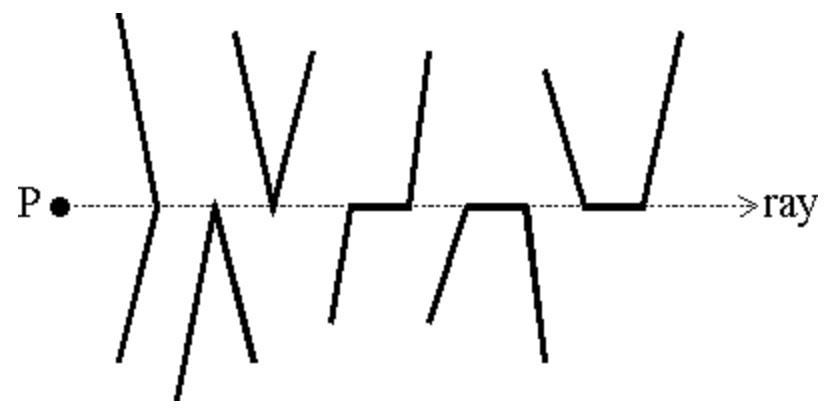
\includegraphics[width=.5\linewidth]{figures/fig11.png}
  \label{fig:12}
  \caption{An edge case for crossing number method which must be avoided}
\end{figure}

One can use the following edge crossing rules to avoid the problems that occurred at the figure.

\textbf{Edge Crossing Rules}:
\begin{enumerate}
  \item an upward edge includes its starting endpoint, and excludes its final endpoint
  \item a downward edge excludes its starting endpoint, and includes its final endpoint
  \item horizontal edges are excluded
  \item the edge-ray intersection point must be strictly right of the point P
\end{enumerate}

On the other hand, one can trust the power of randomness and check their points' inclusion
with different random vectors. The most occurring result will give us the correct solution with very high probability.

The following implementation is taken from [4].
\begin{lstlisting}
typedef struct {int x, y;} Point;

cn_PnPoly( Point P, Point V[], int n )
{
    int    cn = 0;    // the  crossing number counter

    // loop through all edges of the polygon
    for (each edge E[i]:V[i]V[i+1] of the polygon) {
        if (E[i] crosses upward as long as Rule 1
         || E[i] crosses downward as long as  Rule 2) {
            if (P.x <  x_intersect of E[i] with y=P.y)   // Rule #4
                 ++cn;   // a valid crossing to the right of P.x
        }
    }
    return (cn&1);    // 0 if even (out), and 1 if  odd (in)

}
\end{lstlisting}

\subsection{Winding Number Method}

The Winding Number Method counts the number of times the polygon winds around 
the point $P$. The point is outside only when this "winding number"$=0$; otherwise, 
the point is inside.

In order to count the number of times the polygon winds around the point $P$, we
will only consider the edges that lie at the left part of the point. 
Subtracting the number of downward edges at the left from the number of upward 
edges at the left will give us the winding number of that point.

\begin{center}
  \begin{figure}[!htb]
    \centering
    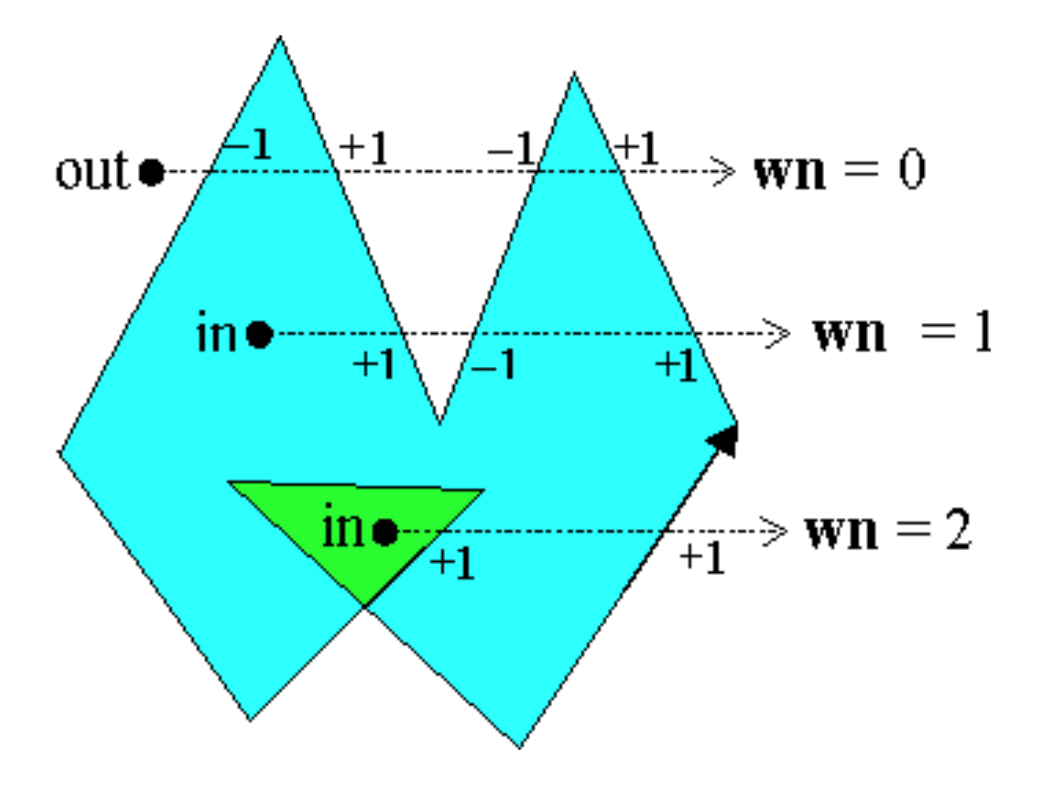
\includegraphics[width=.5\linewidth]{figures/fig12.png}
    \label{fig:13}
    \caption{Illustration of winding number method}
  \end{figure}
\end{center}

We won't dive into the details of this method or give the implementation. However,
it is strongly suggested to see [4].

\section{Convex Hull}
The convex hull of a geometric object (point set, polygon or polygon set) is the
smallest convex set containing that object. There are many equivalent definitions 
for a convex set $S$. The most basic of these is:

\begin{defn}
  A set $S$ is \textbf{convex} if whenever two points $P$ and $Q$ are inside $S$, then the 
  whole line segment $\pmb{PQ}$ is also in $S$.
\end{defn}

\begin{center}
  \begin{figure}[!htb]
    \centering
    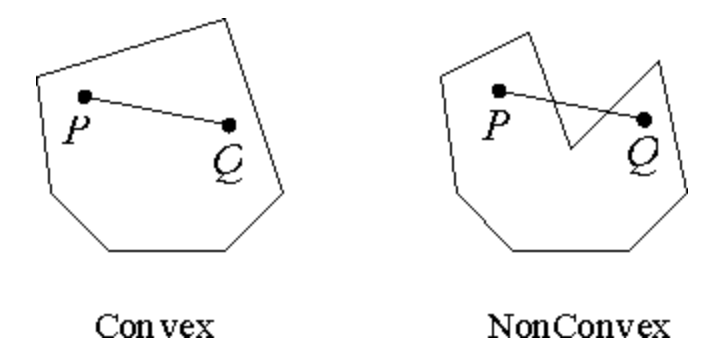
\includegraphics[width=.5\linewidth]{figures/fig13.png}
    \label{fig:14}
    \caption{Examples of convex and non-convex sets}
  \end{figure}
\end{center}

\begin{defn}
  A set $S$ is \textbf{convex} if it is exactly equal to the intersection of all the
  half planes containing it.
\end{defn}

In different dimensions convex sets have different names, for example in 2D it is
convex polygon and in 3D it is polyhedron. However, in this lecture we will only 
work on 2D.

\subsection{Graham-Scan Algorithm}

Our first algorithm is known as Graham-Scan Algorithm due to [5]. Before we discuss the algorithm we will first define a primitive which is required
for this algorithm. As we discussed earlier the area calculation of the triangle has a sign which denotes whether three points in counter-clockwise(CCW) order or clockwise(CW) order. We will use this calculation mechanism to check whether a point lies on the left half-plane of a vector or the right one.

Suppose we have a set of points $S$ and we want to find the convex hull of those
points. We will firstly find the rightmost point from the lowest points of the set.
Let's say that point $P_0$.
This can be done in $O(n)$ time complexity. Then by considering that point as origin
(suppose that we translated points to make this point as origin), we will sort
each point $P$ according to the angle between the $\pmb{P_0P}$ and x-axis in 
increasing order. Then we will be in a situation similar to the following figure.

\begin{center}
  \begin{figure}[!htb]
    \centering
    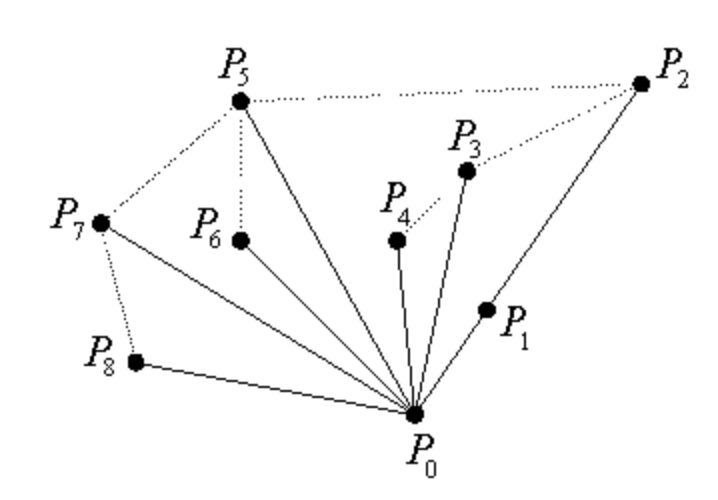
\includegraphics[width=.45\linewidth]{figures/fig14.png}
    \label{fig:15}
    \caption{Points sorted according to their radial angles}
  \end{figure}
\end{center}

When sorting those points one can use trigonometric functions that belong to the programming
environment but this might be inaccurate and inefficient. Instead of trigonometric
functions, one can also use the isLeft function to compare locations of the points
relative to each other. One important trick to speed up the process is that if two points have the same radial angle then nearer one should be ignored since it can not belong to the 
convex hull(why?).

We next iterate through all points in a determined order. We will use a stack data structure
to keep track of which points belong to convex hull. We will start with two points
in the stack $P_0$ and $P_1$. Then at $k^{th}$ step of iterations we will look 
at the relative position of the next point with respect to the vector determined by the top two points of the stack. If the new point lies at the left part of that vector
then that point will be added to the top of the stack. If it lies at the right part of the
vector, then the top of the vector must be removed from the stack until finding such a vector
(Think about why we can eventually find such a vector.). Note that each point 
will be added to the stack at first consideration, and then it may be removed or not.
The following figure illustrates one interesting situation.

\begin{center}
  \begin{figure}[!htb]
    \centering
    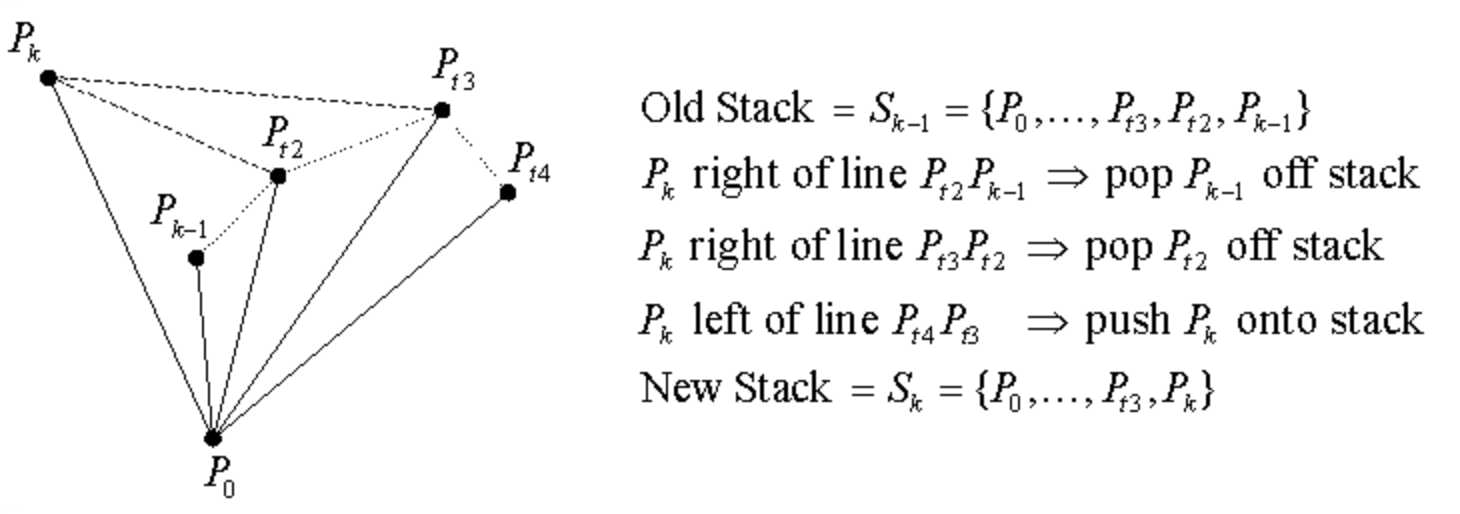
\includegraphics[width=.85\linewidth]{figures/fig15.png}
    \label{fig:16}
    \caption{Example of iterations at stack}
  \end{figure}
\end{center}

\begin{exercise}
  Convince yourself why the algorithm works. 
  Think about what is the importance of having points in increasing radial order.
\end{exercise}

The following implementation is taken from [4].
\begin{lstlisting}
    Input: a  set of points S = {P = (P.x,P.y)}

    Select the rightmost lowest point P0 in S
    Sort S radially (ccw) about P0 as a center {
        Use isLeft() comparisons // see below for the implementation
        For ties, discard the closer points
    }
    Let P[N] be the sorted array of points with P[0]=P0

    Push P[0] and P[1] onto a stack OMEGA

    while i < N
    {
        Let PT1 = the top point on OMEGA
        If (PT1 == P[0]) {
            Push P[i] onto OMEGA
            i++     // increment i
        }
        Let PT2 = the second top point on OMEGA
        If (P[i] is strictly left of the line  PT2 to PT1) { 
            Push P[i] onto OMEGA
            i++     // increment i
        }
        else
            Pop the top point PT1 off the stack
    }

    Output: OMEGA = the convex hull of S.
\end{lstlisting}

\subsection{Andrew's Monotone Chain Algorithm}

Andrew's algorithm [6] is very similar to the previous one but in comparison to 
Graham's algorithm, this algorithm sorts the points according to their coordinates.

Suppose as in the previous case, you have a set of points $S$ and you want to 
find the convex hull containing these points. Firstly, sort all the points
by increasing $x$ and then $y$ (when there are points with same $x$ coordinates) 
coordinate values. Let $P_{min,min}$ be the point with minimum $x$ coordinate and 
from those points minimum $y$ coordinate. And similarly define $P_{min,max}$,
$P_{max,min}$, $P_{max,max}$. Note that sometimes $P_{min,max} = P_{min,min}$
and $P_{max,min} = P_{max,max}$. Define two lines $L_{min}$ which connects 
$P_{min,min}$ and $P_{max,min}$ and $L_{max}$ connecting $P_{min,max}$ and $P_{max,max}$.
An example situation can be shown in the following figure.

\begin{center}
  \begin{figure}[!htb]
    \centering
    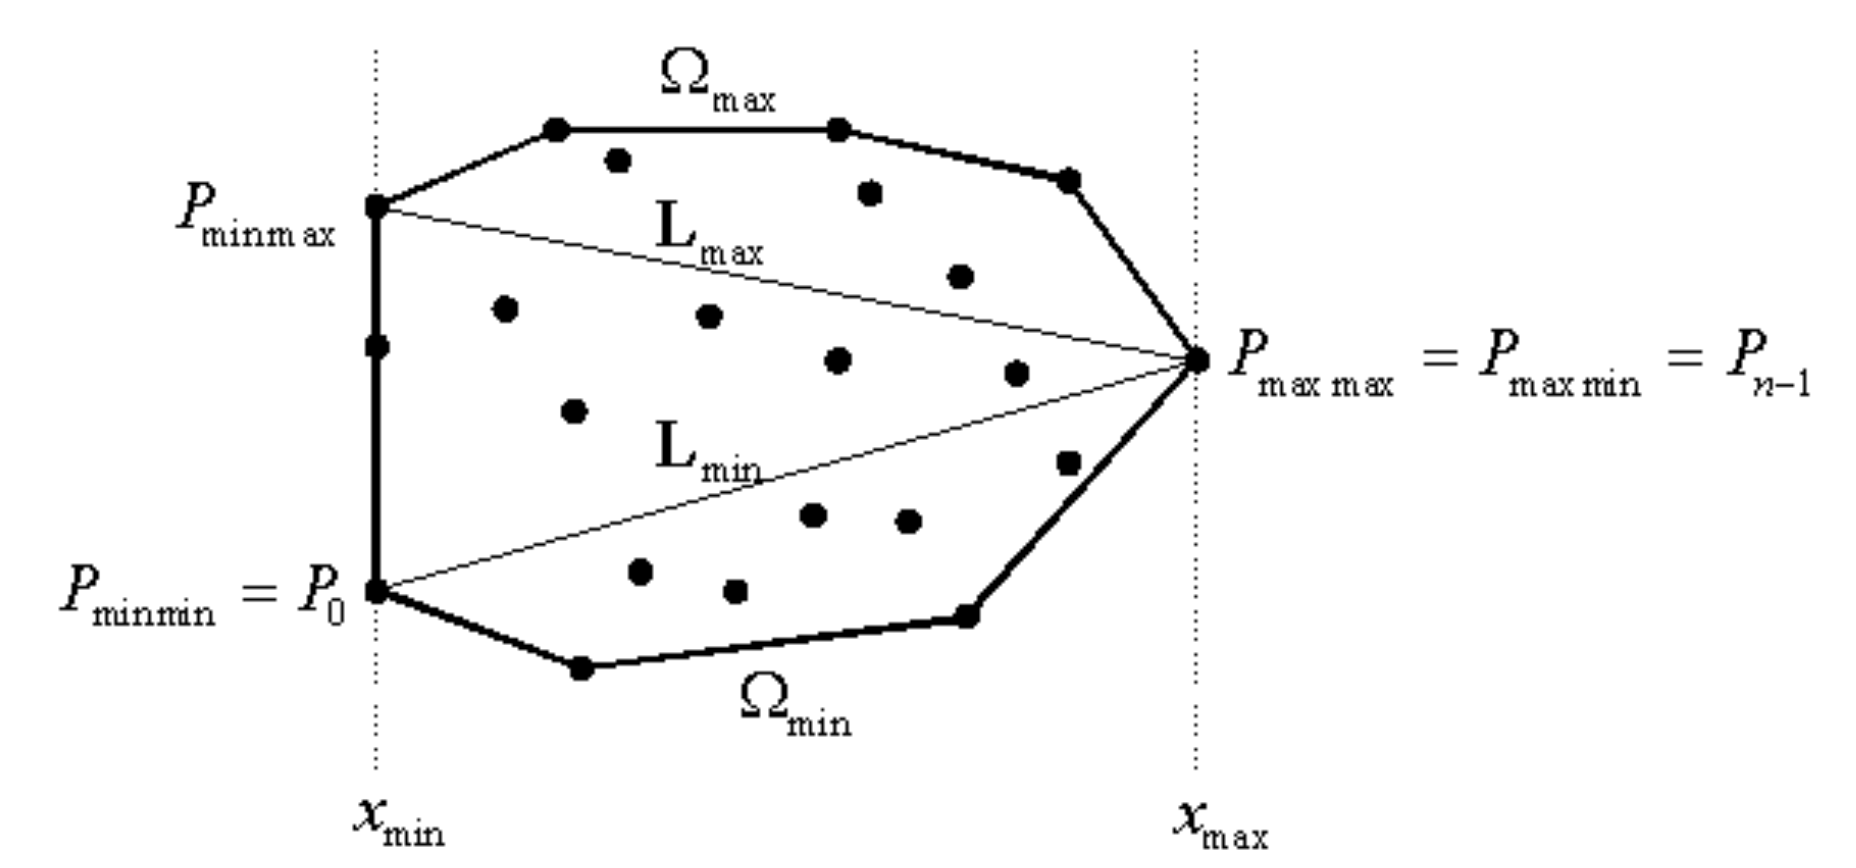
\includegraphics[width=.7\linewidth]{figures/fig16.png}
    \label{fig:17}
    \caption{Illustration of Andrew's Monotone Chain Algorithm}
  \end{figure}
\end{center}

Now, the aim of the algorithm is finding upper hull $\Omega_{max}$ which is above the $L_{max}$
and finding lower hull $\Omega_{min}$ which is below the $L_{min}$. Then the 
convex hull $\Omega$ will be constructed by connecting these two hulls.

While finding the upper and lower hull we will iterate the stack idea we have used in
the previous algorithm to keep of track which points belong to hull. For the $\Omega_{max}$,
we will iterate the process in increasing $x$ order and consider each point if it lies above the
$L_{max}$. When considering a point we will check whether a point lies at right
side of the line determined by the top two elements of the stack (similar to the previous algorithm).
Using this comparison we will add the new point to the stack or remove the top points 
from the stack until we find such a case. An analogous version of this can be defined for lower hull as well.

The following implementation is taken from [4].
\begin{lstlisting}
// Copyright 2001 softSurfer, 2012 Dan Sunday
// This code may be freely used and modified for any purpose
// providing that this copyright notice is included with it.
// SoftSurfer makes no warranty for this code, and cannot be held
// liable for any real or imagined damage resulting from its use.
// Users of this code must verify correctness for their application.
 

// Assume that a class is already given for the object:
//    Point with coordinates {float x, y;}
//===================================================================
 

// isLeft(): tests if a point is Left|On|Right of an infinite line.
//    Input:  three points P0, P1, and P2
//    Return: >0 for P2 left of the line through P0 and P1
//            =0 for P2 on the line
//            <0 for P2 right of the line
//    See: Algorithm 1 on Area of Triangles
inline float isLeft( Point P0, Point P1, Point P2 )
{
    return (P1.x - P0.x)*(P2.y - P0.y) - (P2.x - P0.x)*(P1.y - P0.y);
}


// chainHull_2D(): Andrew's monotone chain 2D convex hull algorithm
//     Input:  P[] = an array of 2D points 
//                  presorted by increasing x and y-coordinates
//             n =  the number of points in P[]
//     Output: H[] = an array of the convex hull vertices (max is n)
//     Return: the number of points in H[]
int chainHull_2D( Point* P, int n, Point* H )
{
    // the output array H[] will be used as the stack
    int    bot=0, top=(-1);   // indices for bottom and top of the stack
    int    i;                 // array scan index

    // Get the indices of points with min x-coord and min|max y-coord
    int minmin = 0, minmax;
    float xmin = P[0].x;
    for (i=1; i<n; i++)
        if (P[i].x != xmin) break;
    minmax = i-1;
    if (minmax == n-1) {       // degenerate case: all x-coords == xmin
        H[++top] = P[minmin];
        if (P[minmax].y != P[minmin].y) // a  nontrivial segment
            H[++top] =  P[minmax];
        H[++top] = P[minmin];            // add polygon endpoint
        return top+1;
    }

    // Get the indices of points with max x-coord and min|max y-coord
    int maxmin, maxmax = n-1;
    float xmax = P[n-1].x;
    for (i=n-2; i>=0; i--)
        if (P[i].x != xmax) break;
    maxmin = i+1;

    // Compute the lower hull on the stack H
    H[++top] = P[minmin];      // push  minmin point onto stack
    i = minmax;
    while (++i <= maxmin)
    {
        // the lower line joins P[minmin]  with P[maxmin]
        if (isLeft( P[minmin], P[maxmin], P[i])  >= 0 && i < maxmin)
            continue;           // ignore P[i] above or on the lower line

        while (top > 0)         // there are at least 2 points on the stack
        {
            // test if  P[i] is left of the line at the stack top
            if (isLeft(  H[top-1], H[top], P[i]) > 0)
                 break;         // P[i] is a new hull  vertex
            else
                 top--;         // pop top point off  stack
        }
        H[++top] = P[i];        // push P[i] onto stack
    }

    // Next, compute the upper hull on the stack H above  the bottom hull
    if (maxmax != maxmin)      // if  distinct xmax points
         H[++top] = P[maxmax];  // push maxmax point onto stack
    bot = top;                  // the bottom point of the upper hull stack
    i = maxmin;
    while (--i >= minmax)
    {
        // the upper line joins P[maxmax]  with P[minmax]
        if (isLeft( P[maxmax], P[minmax], P[i])  >= 0 && i > minmax)
            continue;           // ignore P[i] below or on the upper line

        while (top > bot)     // at least 2 points on the upper stack
        {
            // test if  P[i] is left of the line at the stack top
            if (isLeft(  H[top-1], H[top], P[i]) > 0)
                 break;         // P[i] is a new hull  vertex
            else
                 top--;         // pop top point off  stack
        }
        H[++top] = P[i];        // push P[i] onto stack
    }
    if (minmax != minmin)
        H[++top] = P[minmin];  // push  joining endpoint onto stack

    return top+1;
}
\end{lstlisting}

\begin{exercise}
  Convince yourself why algorithm works. 
  Think about what is the importance of having in increasing $x$ order.
\end{exercise}

\section{Rotating Calipers}
%REF !!! Solving Geometric Problems with the Rotating Calipers
%REF2 !!! http://digitool.library.mcgill.ca/webclient/StreamGate?folder_id=0&dvs=1553106458024~274&usePid1=true&usePid2=true
%REF SHAMOS

Let $\Omega = (p_1, p_2, \cdots p_n)$ be a convex polygon whose points are in clockwise order
and no three consecutive points are co-linear(lie at the same line). Our aim is finding
the diameter of the polygon $\Omega$. The diameter of a polygon can be written as
$$ diam(\Omega) = \max_{p,q \in \Omega}\{d(p,q)\} $$ 
A line L is a line of support of $\Omega$ if the interior of $\Omega$. lies completely to one side
of L. Following figure illustrates two parallel lines of support. 

\begin{thm}
The diameter of a convex polygon $\Omega$ is the greatest distance between 
parallel lines of support of $\Omega$.
\end{thm}

For the proof, please see the [REF2].

A pair of vertices $p_i$ and $p_j$ are an antipodal pair if they admit parallel lines of support. The algorithm of Shamos [7] generates all O(n) antipodal pairs of vertices and selects the pair with the largest distance as the diameter-pair. The procedure resembles rotating 
a pair of dynamically adjustable calipers once around the polygon. 
Consider the following figure. 
To initialize the algorithm in a direction such as the x-axis is chosen and the 
two antipodal vertices $p_i$ and $p_j$ can be found in O(n) time 
(points with max x coordinate and min x coordinate).
To generate the next antipodal pair we consider the angles that the lines 
of support at $p_i$ and $p_j$ make with edges $\pmb{p_ip_{i+1}}$ and $\pmb{p_jp_{j+1}}$, respectively. 
Let angle $\theta_j < \theta_i$. Then we rotate the lines of support by an angle $\theta_j$, 
and $p_{j+1}$, $p_i$ becomes the next antipodal pair. This process is continued until
we come full circle to the starting position. 
In the event that $\theta_j = \theta_i$ three new antipodal pairs are generated.

\begin{center}
  \begin{figure}[!htb]
    \centering
    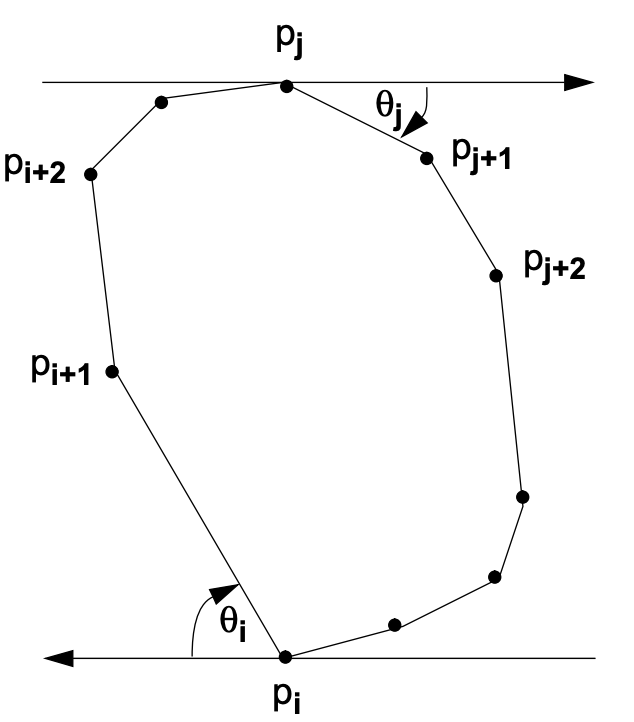
\includegraphics[width=.5\linewidth]{figures/fig17.png}
    \label{fig:18}
    \caption{Illustration of an iteration of rotating calipers algorithm}
  \end{figure}
\end{center}

In implementation, we will start with a random point and find its antipodal pair. Then at each step we will compare the angles between the line of supports and next edges of the polygon for both antipodal pair. Then we will rotate our calipers (pair of support lines) with the minimum angle. In this case one of our line of support will contain an edge of the polygon. This process will be terminated when a full cycle is completed. One can see [14] for C++ implementations of the algorithm.
% https://ideone.com/FxjD9D
% [REF2] http://digitool.library.mcgill.ca/webclient/StreamGate?folder_id=0&dvs=1553106458024~274&usePid1=true&usePid2=true


\subsection{Applications}
In this section, we will list some problems which can be solved by using 
rotating calipers algorithm. A curious reader may consult to [8].
\begin{itemize}
  \item \textbf{The smallest area enclosing rectangle}: can be solved by using two
  pairs of calipers perpendicular to each other.
  \item \textbf{The maximum distance between two convex polygons}: can be solved by
  finding the line of supports for each polygon and iterate rotating idea similar to
  diameter problem.
  \item \textbf{Merging Convex Hulls}: with using calipers idea this can be done
  in O(n) time.
\end{itemize}

\section{Closest Pair}
In this section we will study a well defined problem known as closest pair.
Suppose that you have a set of points $\{p_1,\cdots,p_n\}$ find the pair of points $\{p_i,p_j\}$
that are closest together. Or formally,
$$ d(p_i, p_j) \leq d(p_t, p_k) \ \ \forall t,k \in \{1,\cdots k\} \text{ and } t \neq k $$

A naive approach can be designing algorithm which measures distance between every
pairs. With this approach we can find the closest pair in $O(n^2)$ time complexity.
However, we can improve this running time to $O(n \log n)$.

To find such a pair we will examine two different methods. These two methods 
are very important concepts which can be applied to numerous problems.

\subsection{Divide and Conquer}

Firstly, we will study the Divide and Conquer algorithm which is designed for the closest pair problem, using [9] and [10]. In fact, we are familiar with this concept from the
merge-sort algorithm. The idea is similar; we will divide the set of points to
(almost) equal sized two sets and calculate the desired quantity for those 
sets. Then, we will merge two sets by finding the closest pairs of the combined set.
The algorithm can be summarized as following.

We will use induction to build up our algorithm. For the base case, 
if we have a set of size $2$ then the result will be the only pairs. 
Suppose that we have an algorithm which finds desired pair for a set of 
size less than $n$. Our divide phase makes use of this sub-solver.

Firstly, we will sort all the points according to their x coordinates. Then, 
we will find a line L where (almost) half of the points lie at the left side 
of the line. Then we will use the sub-solver to find the distance $d_{left}$
of closest pair of the left part and the distance $d_{right}$ of closest pair
of the right part. Each sub-solver will call also another 
sub-solver to find its closest pair recursively.
\begin{center}
  \begin{figure}[]
    \centering
    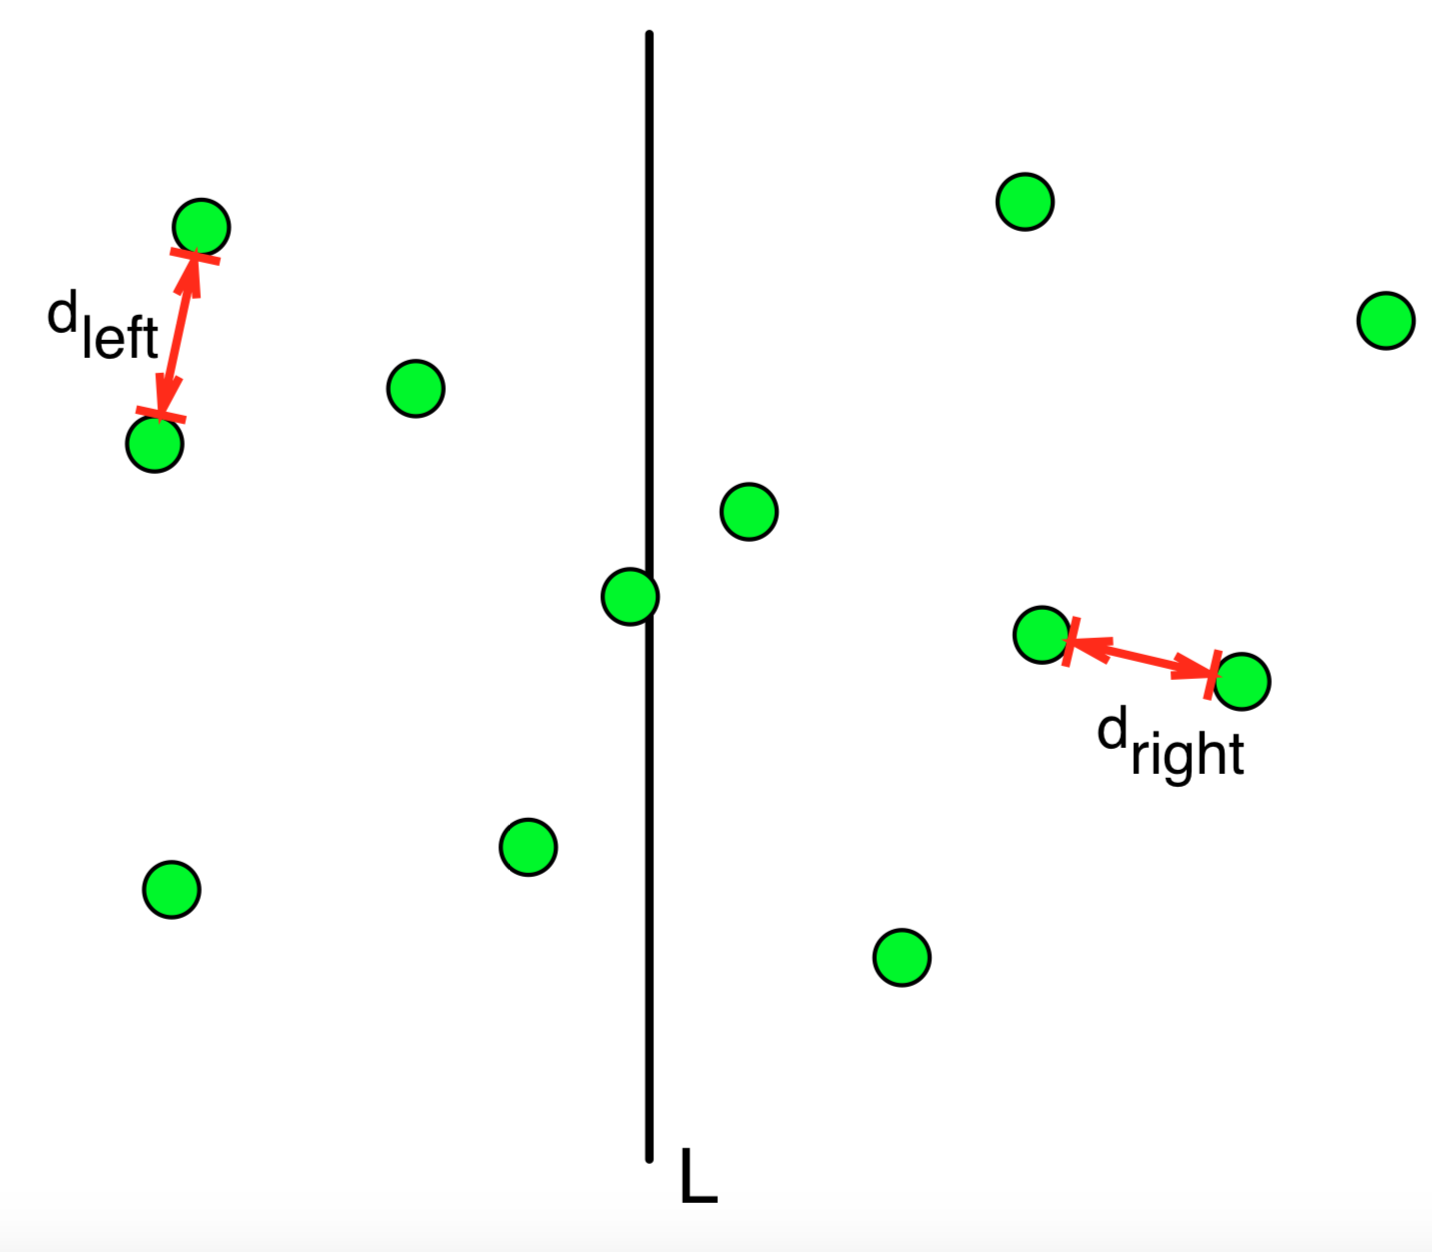
\includegraphics[width=.5\linewidth]{figures/fig19.png}
    \label{fig:20}
    \caption{Divide phase of the algorithm}
  \end{figure}
\end{center}
Next phase is conquer or sometimes called merge phase. At the beginning of this
phase we will set $d=\min\{d_{left}, d_{right}\}$. $d$ would be the answer,
except maybe $L$ split a close pair. Then, we need to deal with the 
near points to $L$. It is obvious that we do not need to consider points 
which are $d$ unit far from $L$ since they can not produce any closer pair.
Then we will look the points which lie inside of the $2d$ width strip around the
$L$.

\begin{center}
  \begin{figure}[!htb]
    \centering
    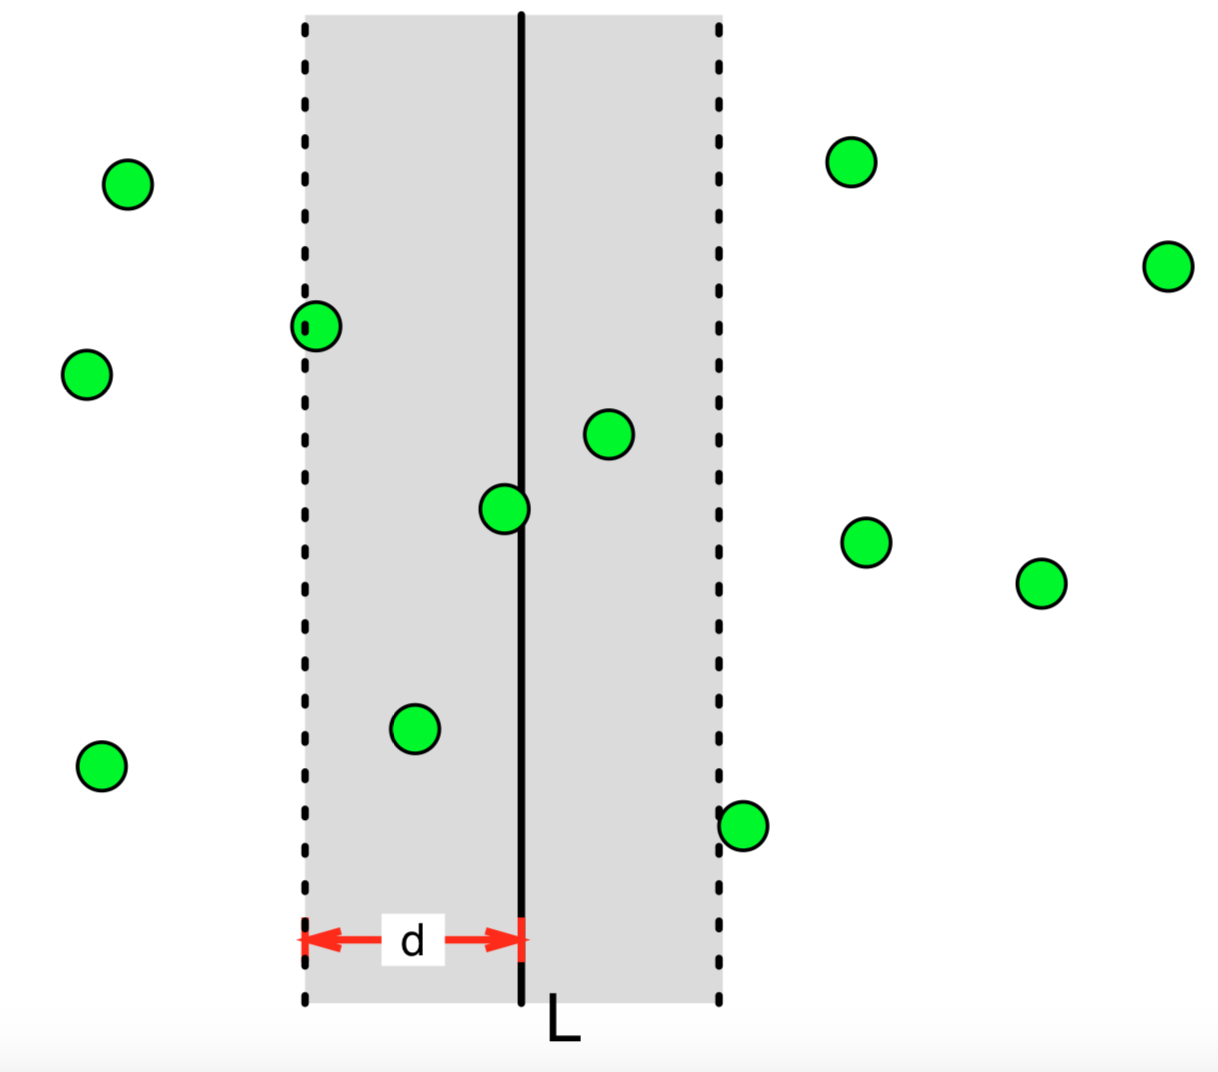
\includegraphics[width=.5\linewidth]{figures/fig20.png}
    \label{fig:21}
    \caption{Merge phase and strip around line $L$}
  \end{figure}
\end{center}

Let $S_y$ be an array of the points in that region, sorted by 
decreasing $y$-coordinate value. The bad case is the strip might contain
all points; then we can not try every pair which can be obtained from $S_y$.
However, the following theorem helps us to avoid this situation.

\begin{thm}
  Suppose $S_y=\{p_1,\cdots,p_m\}$. If $d(p_i,p_j)<d$ then $j-i\leq15$.
\end{thm}

In other words, if two points in $S_y$ are close enough in the plane, 
they are close in the array $S_y$. Then for each point we can look for 
a constant amount of other points to find our desired pair.

\begin{proof}
  Suppose that we divided the region up into squares with sides of length $d/2$.
  Then, each box contains at most $1$ point (why?). 
  
  \begin{center}
    \begin{figure}[!htb]
      \centering
      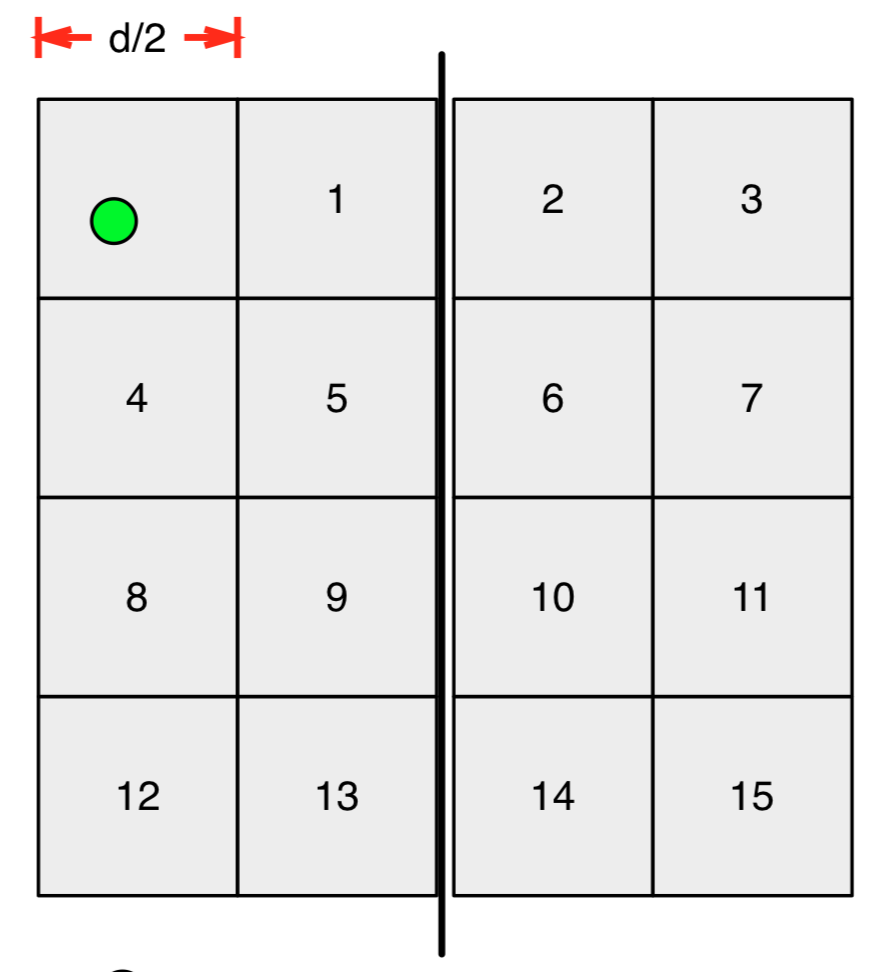
\includegraphics[width=.5\linewidth]{figures/fig21.png}
      \label{fig:22}
      \caption{Line strip divided into squares}
    \end{figure}
  \end{center}

  If $2$ points are separated
  by $>15$ indices, then at least $3$ full rows separate them. However, 
  the height of $3$ rows is $3d/2$ which is bigger than $d$. So the two points
  are farther than $d$ apart.
\end{proof}

\begin{exercise}
  Try to improve the constant $15$ in the theorem.
\end{exercise}

The following implementation is taken from [9].
\begin{lstlisting}
ClosestPair(Px, Py):
  if |Px| == 2: return dist(Px[1],Px[2]) // base
  d1 = ClosestPair(FirstHalf(Px,Py)) // divide
  d2 = ClosestPair(SecondHalf(Px,Py))
  d = min(d1,d2)
  Sy = points in Py within d distance of L // merge
  For i = 1,...,|Sy|:
    For j = 1,...,15:
        d = min( dist(Sy[i], Sy[j]), d )
Return d
\end{lstlisting}

% CODE with $O(n log^2 n)$
% https://www.geeksforgeeks.org/closest-pair-of-points-using-divide-and-conquer-algorithm/

One can merge two regions by an algorithm similar to merge-sort to obtain 
$O(n)$ merging time complexity. Since we can divide sets into sub-sets at most 
$O(\log n)$ depth recursion and at each depth we do operations with $O(n)$ 
time complexity. Complexity of the algorithm is the same with merge sort.

\subsection{Line Sweep}
As we mentioned above, the algorithmic technique we shall use is the 
line sweep method. This means that we will be sweeping a vertical line 
across the set of points, keeping track of certain data, and performing 
certain actions every time a point is encountered during the plane sweep.
As we sweep the line, we will maintain the following data:
\begin{itemize}
  \item The closest pair among the points encountered
  \item The distance d between the points in the above pair
  \item All points within a strip of distance d to the left of the sweep 
  line (see the next figure). These points will be stored in an ordered set D 
  (sorted by their y-coordinates)
\end{itemize}

\begin{center}
  \begin{figure}[!htb]
    \centering
    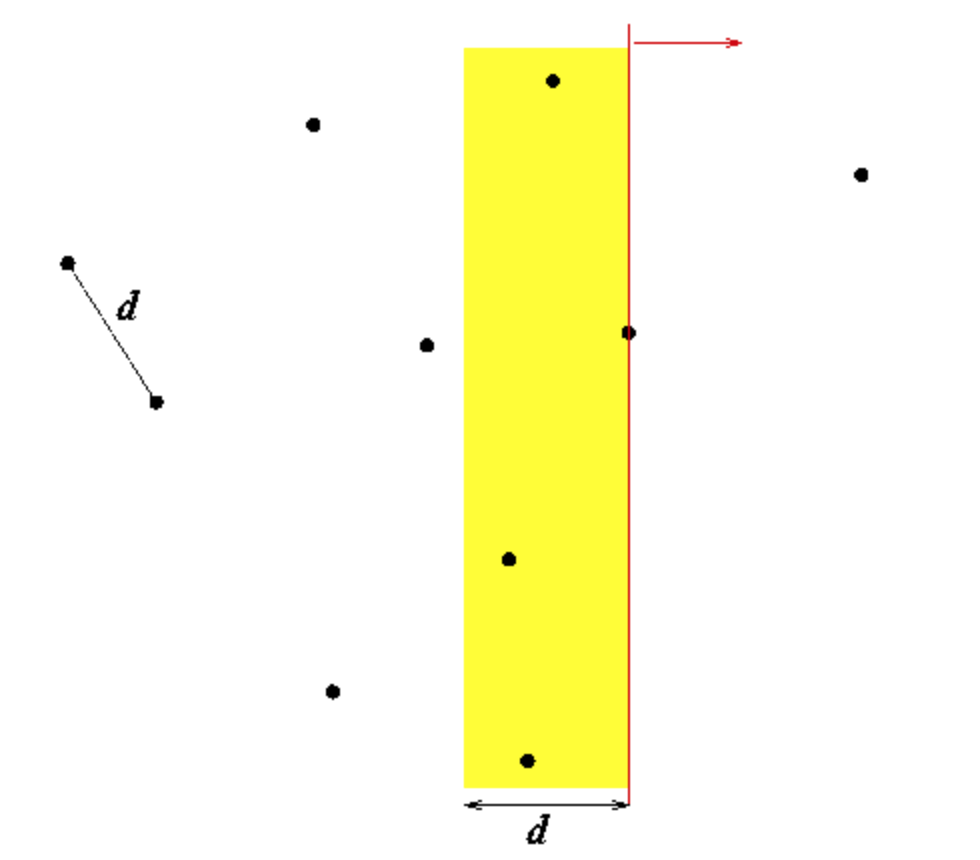
\includegraphics[width=.5\linewidth]{figures/fig22.png}
    \label{fig:23}
    \caption{Illustration of sweep-line method where active points are colored yellow}
  \end{figure}
\end{center}

Now, every time the sweep line encounters a point p, we will perform the 
following actions:
\begin{enumerate}
  \item Remove the points further than d to the left of p from the ordered set D that is storing the points in the strip.
  \item Determine the point on the left of p that is closest to it
  \item If the distance between this point and p is less than d (the current minimum distance), then update the closest current pair and d.
\end{enumerate}

Steps 1 and 3 need no further elaboration, but step two is a little unclear.
It might seem like a method with $O(n)$ time complexity for each encountered point.
However, as in the previous case we can consider only the constant amount of points
lying at left side of the line.

\begin{exercise}
  Think about why this algorithm works. You can see [11] 
  for the proof of correctness.
\end{exercise}


The following implementation is taken from [12].
\begin{lstlisting}
#define x first
#define y second

Following implementation is taken from [9].
typedef pair<long long, long long> pll;
    ...
set <pll> boundingBox;
boundingBox.insert(points[0]); //Points have been already sorted by x-coordinate
for (int i = 1; i < numPoints; i++)
{
    while ((left < i) && (points[i].x - points[left].x > shortestDistSoFar))
    {
        boundingBox.erase(points[left]);
        left++;
    }

    for (auto it = boundingBox.lower_bound(pll(points[i].y - shortestDistSoFar, points[i].x - shortestDistSoFar)); it != boundingBox.end() && it->y <= points[i].y + shortestDistSoFar; it++)
    {
        if (dist(*it, points[i]) < shortestDistSoFar)
        {
            shortestDistSoFar = dist(*it, points[i]);
            best1 = *it;
            best2 = points[i];
        }
    }
    boundingBox.insert(points[i]);
}
\end{lstlisting}

Besides the problem of closest pair, Line-Sweep method has many different applications and it is very useful technique to solve different kinds of geometric problems. In order to see different applications of this technique one can see the excellent blog post of Bruce Merry [12]

\newpage
\begin{thebibliography}{11}
  \bibitem{1}
  Wong Yan Loi, MA1104 Multivariable Calculus Lecture Notes
  \bibitem{2}
  Stewart,J., Calculus, Brooks/Cole., 5th edition, 2003
  \bibitem{3}
  \url{https://www.wikiwand.com/en/Metric_space}
  \bibitem{4}
  \url{http://geomalgorithms.com/}
  \bibitem{5}
  Graham, R.L. (1972). "An Efficient Algorithm for Determining the Convex Hull of a Finite Planar Set", Information Processing Letters. 1 (4): 132–133. 
  \bibitem{6}
  A. M. Andrew. (1979). "Another Efficient Algorithm for Convex Hulls in Two Dimensions", Info. Proc. Letters 9, 216-219.
  \bibitem{7}
  Shamos, Michael (1978). "Computational Geometry" (PDF). Yale University. pp. 76–81.
  \bibitem{8}
  Toussaint, Godfried T. (1983). "Solving geometric problems with the rotating calipers". Proc. MELECON '83, Athens. CiteSeerX 10.1.1.155.5671
  \bibitem{9}
  \url{https://www.cs.cmu.edu/~ckingsf/bioinfo-lectures/closepoints.pdf}
  \bibitem{10}
  Kleinberg, Tardos, (2005). "Algorithm Design". Section 5.4. Addison-Wesley Longman Publishing Co., Inc.
  \bibitem{11}
  \url{https://www.cs.mcgill.ca/~cs251/ClosestPair/ClosestPairPS.html}
  \bibitem{12}
  \url{https://www.topcoder.com/community/competitive-programming/tutorials/line-sweep-algorithms/}
  \bibitem{13}
  \url{https://stackoverflow.com/questions/27674554/understanding-specific-implementation-of-sweep-line-closest-pair}
  \bibitem{14}
  \url{https://ideone.com/FxjD9D}

\end{thebibliography}        
\end{document}